\documentclass{article}
\setcounter{secnumdepth}{0}
%[a4paper, 11pt]
\usepackage{comment} % enables the use of multi-line comments (\ifx \fi) 
\usepackage{fullpage} % changes the margin

\usepackage{graphicx}
%\usepackage{lscape}
%\usepackage{rotating}
\usepackage{pdflscape}
\usepackage{wrapfig}
\usepackage{gensymb}
\usepackage{graphicx} 
\usepackage[utf8]{inputenc}
\usepackage{siunitx}
\usepackage{amssymb}
\usepackage{amsmath}

\renewcommand{\labelenumii}{\theenumii}
\renewcommand{\theenumii}{\theenumi.\arabic{enumii}.}

\usepackage{enumitem}
\usepackage{subcaption}
%\usepackage[]{algorithm2e}
%\usepackage{pgffor}
\usepackage[T1]{fontenc}
\usepackage{xcolor}

\newcommand{\CMwidth}{-1.7cm}
\newcommand{\CMheight}{2.7cm}

\usepackage{hyperref}

\hypersetup{
	colorlinks=true,
	linkcolor=black,
	citecolor=black,
	filecolor=blue,
	menucolor=black,
	urlcolor=blue
}


\setcounter{secnumdepth}{5}% Include \subsubsection in ToC

\def\changemargin#1#2{\list{}{\rightmargin#2\leftmargin#1}\item[]}
\let\endchangemargin=\endlist 

\begin{document}
%Header-Make sure you update this information!!!!
%\noindent
%\large\textbf{Post/Pre-Lab X Report} \hfill \textbf{FirstName LastName} \\
%\normalsize ECE 100-003 \hfill Teammates: Student1, Student2 \\
%Prof. Oruklu \hfill Lab Date: XX/XX/XX \\
%TA: Adam Sumner \hfill Due Date: XX/XX/XX

\title{Dissertation: Hybrid Methods for Finite Element Meshing}
\author{Jack Bradbrook (psyjb4)}
\date{April 5, 2017}
\maketitle

\tableofcontents

\newpage


\section{Introduction}

The overall aim of this project is to perform the task of refining a Finite Element Mesh (FEM) using a stress based method as is typical of FEM refinement in conjunction with an approach that uses techniques from Artificial Intelligence and Machine Learning. It should be possible to reason about the quality of a mesh produced using both methods analytically in order to evaluate the success of the approach and potential for continued use.\\

\noindent
Finite Element Analysis (FEA) is a method widely used across different engineering domains to simulate structures under certain conditions. The method works by taking a geometry defined in continuous terms, discretize it into a mesh system before calculating the property values for each of the discrete elements. This allows engineers to observe the effect the conditions have on the entire structure, see figure 1. \\ 

\noindent
The success of the project will be determined by implementation of a system that is able to combine the two approaches described above in order to refine a mesh to of a quality comparable to that of a successful stress based method.



\section{Motivation and Background}
Over the past forty years FEA has emerged as a prominent technology for simulating complex real world engineering problems \cite{cite0, DolsakPaper94}. FEA works by solving a system of differential equations with each equation representing a single element in a geometric mesh. By doing this FEA is able to generate highly accurate approximations for the properties of complex physical systems \cite{DolsakPaper94} \cite{IntroductionToFE}. The method can also be highly computationally expensive with the complexity typically increasing exponentially with the model size \cite{DolsakPaper94}. Analysis therefore proves to be highly time consuming and costly for individuals and organisations to conduct \cite{ConsultRuleIntelltSystemFE}. \cite{cite03}\\


\subsection{Properties of Finite Element Models}
Although this is a computer science as opposed to a mechanical engineering dissertation it's still important to briefly outline the general principals and properties that underpin the FE method in order to have a general appreciation for how the design and evaluation of the final software system was conducted. \\ 

\noindent
Finite Element Models have several key properties that need to be specified by the engineers who create them, the configuration of these properties greatly determine the results obtained from the models execution. The first of these properties that an FE model posesses is the mesh. The mesh is constructed out of nodes, points which act as intersections between the second component- elements which are either a polygon or a polyhedron between the nodes. Nodes and elements are important concepts as they provide the theoretical framework for reasoning about the other properties of a mesh and hence the overall quality of the model \cite{IntroductionToFE}.\\ 

\noindent
In addition to the nodes and elements FE models also contain inputs and constraints. Inputs can be thought of as the phenomena from the outside world which is acting on the structure and consequently inducing some kind of physical effect on it. Inputs are used by engineers to model the conditions under which the structure will be expected to perform under when it is manufactured and enters operation. \\

% elements can be different types which have different types, typical types
% triangles and squares. 

\noindent
Constraints are another fundamental concept that describe where the model is attached to the outside world. When computing stresses induced through the model there needs to be an area through which the stresses are assumed to leave. FEA is only able to calculate the path of the stresses through the model and thus the overall stress at given points using the law of conservation of energy i.e. energy cannot be created or destroyed meaning that any energy provided to the system as input through for example force needs a means by which to leave it, the constraint. \\

\noindent
For example in figure 6 showing a suspension bridge model, the simulation is to be run with the forces are induced upon the cables and the towers in the negative x direction as represented by the green vectors. The corresponding constraint area through which the force must leave is specified as the base of each bridge pillar and represented by multiple red arrows on each corresponding corner.\\

\noindent
The final piece of information needed in order to calculate the stresses through the model is material data. Material data is associated with the models elements and is usually defined using two main parameters which are:

\begin{itemize}
\item Youngs Modulus - The ratio of stress over strain for a given material, i.e. for an amount of internal force endured by a material how much does it deform, a material such as rubber therefore has a low value for Young's modulus while diamond has a high value \cite{YoungsModulus}.

\item Poissons ratio - Amount of deformation that occurs perpendicular to the force that is applied to the material.
\end{itemize}

\noindent
For the sake of simplicity all structures used to evaluate the final software solution have assumed steel as their material property. Steel is a pretty common material used within manufacturing of many mechanical components and does not exhibit any abnormal properties. This is beneficial for evaluation as it removes variability in the results that could arise from selecting a more complex material.

\subsection{Limitations and general considerations}
\noindent
An important consideration when conducting FEA is the trade-off of a models accuracy against the time in which it can be solved. A major variable determining this trade-off is the models mesh structure which discretizes the problem so that simulation can be run on it. A mesh that is finer is more computationally expensive but also produces results of greater accuracy. It is therefore desirable to generate a mesh which is fine where accuracy is most needed but coarse where it is not \cite{cite04}. \\

\noindent
In every type of analysis that the FE method is used for (thermal, structural, fluid flow, electrical) there is a specific differential equation associated with each of the elements. In order to achieve overall convergence of the model the equations must be solved simultaneously to achieve a value for each of the discrete elements \cite{IntroductionToFE}. For this dissertation project attention will be given specifically to the problem of FEA meshing in the context of static structural analysis where the value calculated across each element is its stress. It makes sense to work on hybrid mesh refinement in the context of static structural analysis as it is likely the most common engineering application of the method and as such has the largest body of research that is relevant \cite{DolsakPaper94}\cite{IntroductionToFE}.\\

\noindent
For engineers the value obtained through computing the stresses under a particular set of conditions is feedback on the quality of their design. Ideally the results from an analysis will provide a good understanding of where the design is weak and how concentrated this weakness is. This information is used to either help verify the designs' quality or alternatively inform changes to its geometry or material properties so as to reduce stress on subsequent analysis \cite{cite06}.\\

\noindent
To understand the gradient of stress within a part of the model the mesh needs to be designed carefully. As each element can only display values calculated from its edge nodes a smooth gradient requires a higher concentration of elements in areas under higher stress. A high quality mesh is therefore considered to have a higher concentration of elements in areas of predicted high stress while retaining lower concentration elsewhere, thereby revealing weaknesses in the design while minimising the models runtime.\\

\noindent
Traditionally the automated mesh refinement process consists of computing stresses for a model with an initial coarse mesh and low computation cost, once rough stresses have been computed the elements in areas of higher stress can be divided recursively into additional elements in order to achieve smoother gradients on further executions \cite{cite03}. Figure 1 shows a mesh which has been refined in an area of higher stress thus providing a clearer indication of a components weakness. \\ 

\noindent
Unfortunately for many large models this method for refining a mesh is still excessively costly \cite{DolsakPaper91}. It is therefore worth investigating use of alternative approaches posed by the field of computer science and artificial intelligence that could support the traditional high stress meshing approach. 

\begin{figure}[h!!]
  \centerline{\includegraphics[width=110mm, scale=0.5]{../Graphics/stressedCorner.png}}
  \caption{Mesh refinement in corner under high stress image source: (\cite{HighStressCorner})}
  \label{fig:boat1}
\end{figure}
\section{Related Work}
Many approaches have so far been taken in an attempt to improve a computer's ability to perform the task of finite element meshing. The following subsections present an overview of the research conducted for the various aspects of the project which are more explicitly outlined under ``Aims and Objectives"

\subsection{Traditional Subdivision Approaches}
Multiple approaches exist for subdividing different types of meshing with the most common being hierarchical refinementent also known as h-refinement and relocation refinement or r-refinement\cite{HandPRefinements} \cite{RRefinement}\\ 

\noindent
\textbf{h-refinement: }
H-refinement is the process of recursively refining a mesh by splitting elements into additional sub elements. This process can be performed for elements with both both triangular and quadrilateral shapes \cite{HandPRefinements}. \\ 

\noindent
\textbf{r-refinement: }
R-refinement is a method which attempts to improve the quality of the stress gradient without the alteration of the mesh element count and thus the computational cost. This is achieved by the relocation of elements within the mesh which effectively increases the size of elements in areas of low stress, while reducing the size in areas where stress is high \cite{RRefinement}.


\subsection{Stress Refinement}
Refining a mesh based on some model parameter is consistent across all types of FE modelling. Execution of a model with a generic mesh is first required so as to obtain a set of results by which further refinement can be targeted. Using unique ids for nodes allows results from the previous iteration to be compared against the mesh and refinement to be focused on those nodes exhibiting a high amount of a specified property \cite{FiniteElementMeshRefinement}.


%A number of methods exist to perform mesh refinement based on a stress gradient for a mesh,


\subsection{Uses of Artificial Intelligence and Machine Learning}

\noindent
Within the domains of AI and machine learning methods such as neural networks \cite{NeuralNetworks}, case based reasoning \cite{caseBasedReasoning} and inductive logic programming \cite{DolsakPaper94} have been adopted to facilitate generation of meshes comparable to that of human experts.  Similarly there has also been effort to combine multiple numerical methods simultaneously for solving re meshing problems \cite{TraditionalHybridRefinement} although effort to combine the two approaches does not appear to have so far been made.\\ 

\noindent
Due to the difficulty of obtaining meshes which hold commercial interest the majority of researchers working in this field have had to resort to the use of training sets developed within academia \cite{DolsakPaper91}. The primary issue associated with this is that often the training data does not exhibit the level of complexity that you would expect in many industrial sectors. Many researchers must accept this as a limitation or agree commercial terms with an organisation in order to gain access to their models \cite{DittmerMeshQualityMet}.\\ 

\noindent
Having reviewed a variety of different AI based applications of FE the use of Inductive Logic Programming (ILP) used by Bojan Dolsak et al is of greatest interest. ILP is a machine learning method first presented by Stephen Muggleton in his 1991 paper ``Inductive Logic Programming" \cite{MuggletonILP}. Muggleton suggests that the traditional approaches of machine learning which rely on use of extensive data sets and statistical analysis are poor in the case of many real world problems for which data is not available \cite{ILPYoutubeLecture}. Muggleton cites Human learning as an example of use of ILP style techniques where understanding of new concepts is achieved not through crunching large volumes of data points but instead  the use of induction on a relatively concise set of background facts and examples obtained from previous life experiances \cite{ILPYoutubeLecture}. \\ 

\noindent
ILP uses three types of input information in order to hypothesise additional facts about the system. These three types of input information are: \\ 

\begin{itemize}
\item Positive examples  of what constitutes an area that is well meshed
\item Negative example of areas that are poorly meshed
\item Background facts
\end{itemize}

\noindent
Using this information ILP is capable of hypothesising rules by determining which rules can exist within the system where given the set of background facts all positive examples are satisfied while few or none of the negative examples are. Although ILP requires a body of additional metadata associated with each mesh this is easier to obtain making ILP a highly practical solution. Along with his publication Muggletons also released his implementation of an ILP algorithm as a program titled ``Golem" \cite{Golem}, Golem was applied by Dolsak to the problem of mesh refinement with a training set of just five meshes \cite{DolsakPaper94}. The resulting rule set when applied to subsequent models was able to correctly classify and re mesh areas with an average accuracy of 78\% for a range of geometries \cite{DolsakPaper94} \cite{appOfILPToFEMeshDesign}. \\

\noindent
Dolsak's choice of metadata for the ILP method to generate mesh rules is based on the classification of edges within the FE model. Dolsak recognises that edges act as an important intersections within the model and as such provide useful items of reference when designing heruristics with which to reason about the model \cite{DolsakPaper94} \cite{appOfILPToFEMeshDesign}.  For example if it is know that an edge has a force applied close to it based on the initial model conditions then other edges that intersect it should be additionally refined \cite{DolsakPaper91} \cite{appOfILPToFEMeshDesign}. \\ 

\noindent
The format of the rules also make them attractive for experimenting with as part of a hybrid method since the method determines how to refine the mesh based on the arrangement of edges. This detail of analysis of the mesh is at a comparable detail to that of a traditional splitting method such as h-refinement which is likely to improve the ease with which the two methods can be combined simultaneously in the latter stages of the project. \\ 

\subsection{Quality metrics}
\noindent
Finally work has also been done on establishing valid metrics for assessing the quality of a mesh automatically \cite{DittmerMeshQualityMet, NeuralNetworks} Metrics for meshes have been researched far more extensively than AI methods due to their use for comparing different stress based refinements. There are also cases of common metrics being used for industrial meshing applications \cite{DittmerMeshQualityMet}. Although there are metrics for assessing a mesh on a global level such as element count score the consensus is that due to the variation in meshes this is less reliable than assessing quality based on the properties of individual elements within the mesh \cite{DittmerMeshQualityMet}. \\

\noindent
Localised metrics associated with the quality of each element have shown to be accurate for predicting the overall quality of a mesh when taking the average for each metric across all elements \cite{DittmerMeshQualityMet}. The quality of an elements shape is important since the stress values which are computed for the area within the element are calculated using the stress values at each of the nodes which enclose it \cite{IntroductionToFE} a mesh containing a large number of distorted elements is therefore likely to yield inaccurate stress results when given to a FE solver such as LISA. Elements are typically deformed near parts of the geometry where its shape simply does not allow a uniform element to be placed, an example of where this has occurred can be seen in figure 2.\\ \\ \\ \\ \\ \\ \\ \\ \\ \\ 

\begin{figure}[!h]
  \centerline{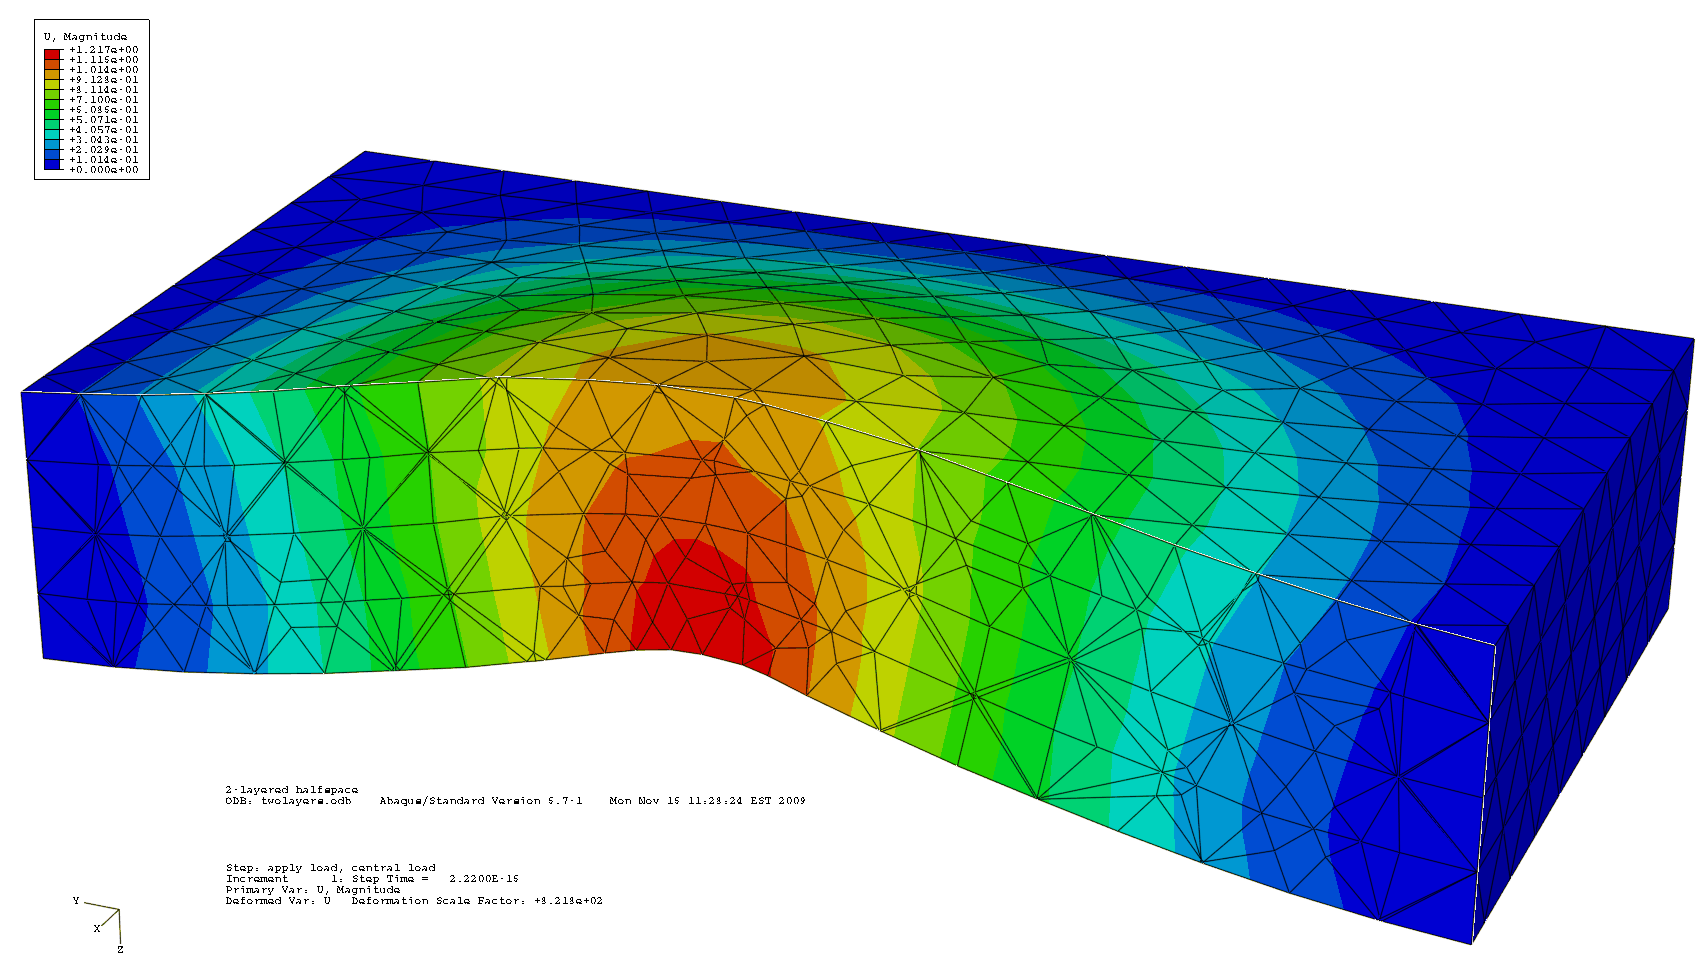
\includegraphics[width=120mm, scale=1]{../Graphics/MeshQualityDeterioration.png}}
  \caption{Example of how elements can be distorted in order to fit a geometry which will result in deterioration of gradient quality (image source: \cite{PoorFEElementShapes})}
\end{figure}

\noindent
Some key shape metrics identified by Dittmer et al include (ideal values are for elements of quadrilateral type as used in  the current prototypes):

\begin{enumerate}[label=\Alph*]
\item Aspect ratio – longest side / shortest side, ideal value is 1
\item Maximum corner angle - widest internal angle to element, ideal is 90\degree
\item Maximum parallel deviation - how skewed the element is, ideal is 0\degree
\end{enumerate}

\section{Description of the work}
\subsection{Aims and Objectives}
The aim of this project was to design, build and analyse a system for refining a mesh by combining a method derived from the fields of AI or machine learning with a method relying purely on information already present in the model. The desirable end result will be a hybrid method of meshing which effectively prioritises those areas of importance whilst incurring a reduced computational cost.\\

\noindent
The project can be broken down into thee main areas of research and implementation which have the following high level objectives:\\ 

\begin{enumerate}[label=\Alph*]

\item Research and implement both a traditional refinement procedure using data present within the model and an approach using techniques from AI developed and used by either industry or academia. These algorithms should be able to run independently on a set of example models.

\item Secondly a process needs to be devised to combine the two re meshing methods to varying degrees. This will make it possible to evaluate and compare the effects of a hybrid meshing against each of the individual methods for a range of models. Through this it should be possible to establish whether or not there is potential benefit to using a hybrid approach and if so to what extent.

\item The third objective will be to research and implement justifiable metrics for assessing the quality of a given mesh, this will allow objective comparisons to be made for the resulting meshes.


% This will allow for a much greater range of hybrid variations to be tried without requiring inspection from an expert. 
\end{enumerate}

\subsection{System specification}
To demonstrate success in achieving the objectives of the project it is important to have traceability from the requirements through to the solution and lastly verification and validation. This section describes the systems initial \textit{functional requirements} (what the system will do) and \textit{non-functional} requirements (its constraints) based upon evaluation of the research conducted in conjunction with discussions with the project supervisor: Dr Jason Atkin. Functional requirements have primarily been listed under their respective high level subsystems that are responsible for encapsulating their functionality. \\ 

\noindent
Although it has not been developed as part of the project the application responsible for solving the finite element models has been included as part of the systems requirements since it highly influences the overall scope of the project and much of the design associated with other subsystems which were developed for the project. \\ 

\subsection{Functional Requirements}

\begin{enumerate}
\item FE integration: System will be able to interface with a third party finite element application

\begin{enumerate}
\item The finite element applications solver must be able to solve a mesh based on its model configuration.
\item The finite element applications solver must be able to execute a model programmatically
\item The finite element applications solver must be able to output stress data at different points on the mesh.
\item The finite element application will provide a graphical representation of the model.
\item It will be possible to manipulate the model that the finite element application uses programmatically.
\item It should be possible to manipulate the model that the finite element application uses from within its graphical user interface.
\end{enumerate}

\item Mesh refinement: System will be able to perform different kinds of finite element mesh refinement

\begin{enumerate}
\item The system will be able to refine a finite element mesh using a stress based refinement method.

\item The system will be able to refine a finite element mesh using a non-stress based refinement method.

\item A non stress based refinement method will adapt the mesh using background information about mesh design which has been previously trained.

\item The system will be able to combine the two methods to produce a coherent mesh which the FE application is able to successfully solve in order to obtain results for stress and displacement.

\item The system will be able to combine both methods to varying degrees that will be performed automatically by the system without direct user intervention.
\item The system will re mesh using both stress and non-stress based refinement using quadrilateral elements.

\item System will adapt weighting associated with each method based upon the metrics computed for the mesh in the systems previous iteration.
\end{enumerate}

\item Quality assessment: System will provide the operator with results about the quality of meshes based on metrics obtained from research.

\begin{enumerate}
\item An assessment will be conducted automatically for every mesh iteration that occurs.

\item System will assess quality based on a variety of metrics to ensure overall robustness of measurement. 

\item The metrics will be computed for both individual element within the model and for the entire mesh.
\end{enumerate}
\end{enumerate}

\subsection{Non-Functional Requirements}


\textbf{Design:} The system architecture will be developed using the object oriented design principals of SOLID to allow for clear interfaces between the different functional components. Functional programming practices will be adopted through use of the .NET Language Integrated Query or LINQ framework. This will help to simplify the code and improve reliability by removing unnecessary state from the program. Where functions and classes are written their length will be kept to a minimum to reduce complexity and allow for reuse wherever possible. \\ 

\noindent
\textbf{Documentation:} The system will be comprehensively documented at both a code level and at an architecture level. At a code level C\# doc comments will be written to provide a comprehensive summary of each function. This will allow the tool Doxygen \cite{Doxygen} to generate a full set of developer documentation upon completion of the software implementation which will be included as an appendix. Ensuring that the majority of information is present within doc comments will also help to promote a reduction of loose comments within the code and hence function size. \\

\noindent
\textbf{General applicability:} In order to demonstrate that hybrid methods are a feasible means of approaching meshing problems the resulting software should be able to successfully execute on a range of models with varying geometry. The range of geometries should be representative of typical structural variation encountered by engineers.
\section{System Design}

\subsection{System Overview}
Determining the overall design of the system was initially hard since it was not clear exactly how many subsystems would be needed to mesh, evaluate and interface with LISA, what was clear was that the system would essentially be performing an optimisation procedure and as such needed to be driven iteratively towards a goal. The variable complexity and uncertainty surrounding the different parts of the project meant ensuring the architecture remained modular with well defined interfaces allowing components to easily be added or modified as the project progressed. \\ 

\begin{figure}[!h]
  \centerline{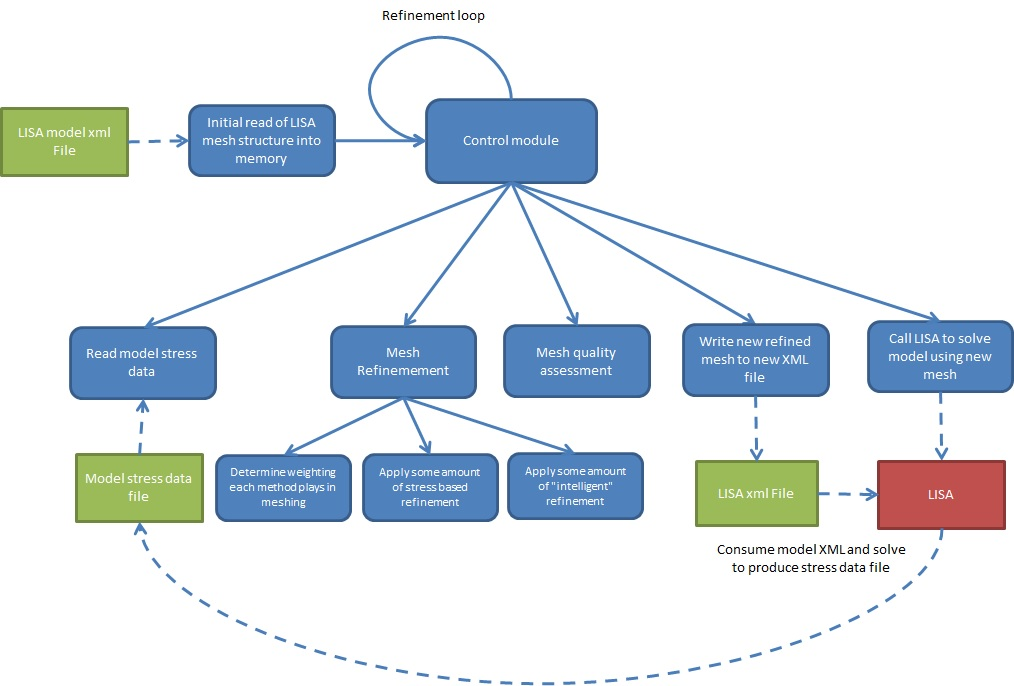
\includegraphics[width=150mm, scale=1]{../Graphics/SystemDesignDiagram.jpeg}}
  \caption{High level design of the system with its different modules}
  \label{fig:h-refinementImp}
\end{figure}


\subsection{Modular Architecture}
The modular architecture was crucial for allowing meshing algorithms and quality metrics to be replaced as necessary. At best the quality of the output could could only be predicted for each method before it was integrated into the system and executed in a range of different scenarios. To have tightly coupled these individual components would have rendered the overall system a failure in the event that any one of them failed. Instead the loose coupling of the architecture has enabled the system to be considered as more of a framework for testing the effects of combining different meshing approaches in order to generate a hybrid method.\\

\noindent
Although the system was highly modular It was also still desirable to maintain an architecture hierarchy so that classes could be developed independently but easily integrated. Composition was therefore generally favoured over inheritance as a means of building the architecture. Static classes and methods were also used when needing to write utility functions that were required by multiple high level subsystems and therefore did no fit especially well into any particular one. Examples of these are generic vector algebra operations such as dot product, matrix determinant and calculating surface normals.

\noindent
At the highest level namespaces were used to break down the class groups appropriately, namespaces also naturally structured as folders within the Visual Studio (VS) solution explorer (see appendix D) which made navigating the project and finding components much easier as the system expanded in size.

%\subsection{Mesh improvement Loop}
%As with many optimisation problems the refinement process is driven iteratively through a loop. Within the main loop all %interfacing with LISA, Mesh refinement and analysis is conducted which results in an updated version of the model that can be %handed to the subsequent iteration.


\subsection{Simulation Data Model}
Writing an API for LISA was the first stage of development for my project for which a design had to be considered. The API was crucial in order to program the more complex aspects using basic operations and avoid having to regularly perform direct string manipulation of the input files in order to manipulate the model. \\

\noindent
When the first re-meshing iteration occurs the system needs to read the input .liml file into an equivalent class model which closely resembles the files schema, diagrams for which can be seen in figure 4 below. Each class in this model contains corresponding data and methods used to represent and manipulate the model. These methods are then used by each of the refinement approaches to easily alter the mesh in a controlled manner. Once the mesh  has been adapted however it is required to be assessed by the modules responsible for validating its quality before finally being written back to a .liml file for LISA to solve on the subsequent iteration. Designing the data model so that it closely resembled the LISA scema not only made the higher level programming less confusing but also made serialisation of the data back to .liml format much simpler  thus reducing the number of bugs arising from inconsistencies between different representations of the same data. \\

\begin{figure}[h!!]
\centering
\begin{subfigure}{.5\textwidth}
  \centering
  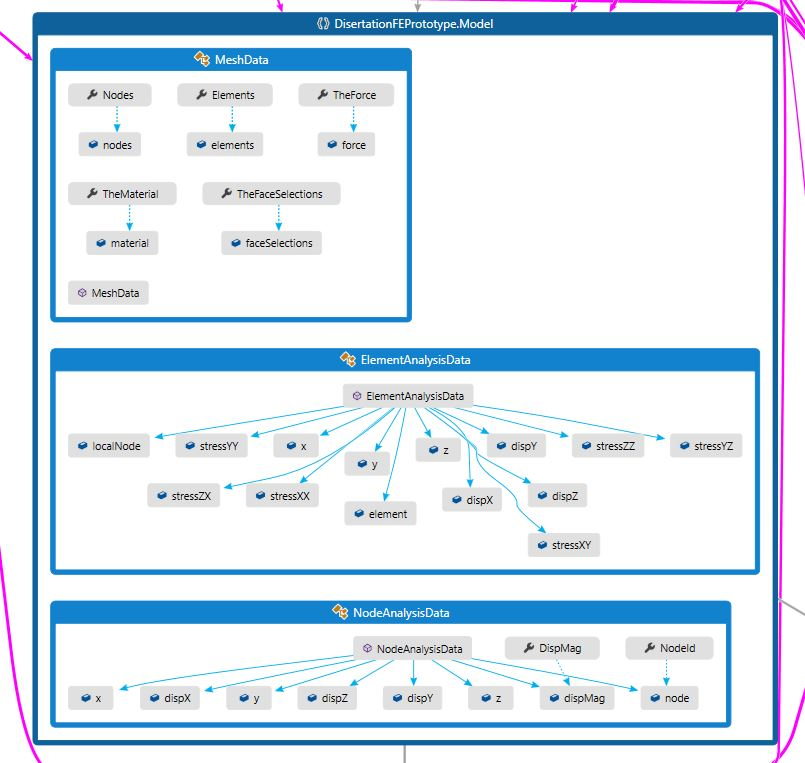
\includegraphics[width=0.9\linewidth]{../Graphics/DissoFEProto-Model.jpg}
  \caption{Model classes}
  \label{fig:sub1}
\end{subfigure}%
\begin{subfigure}{.5\textwidth}
  \centering
  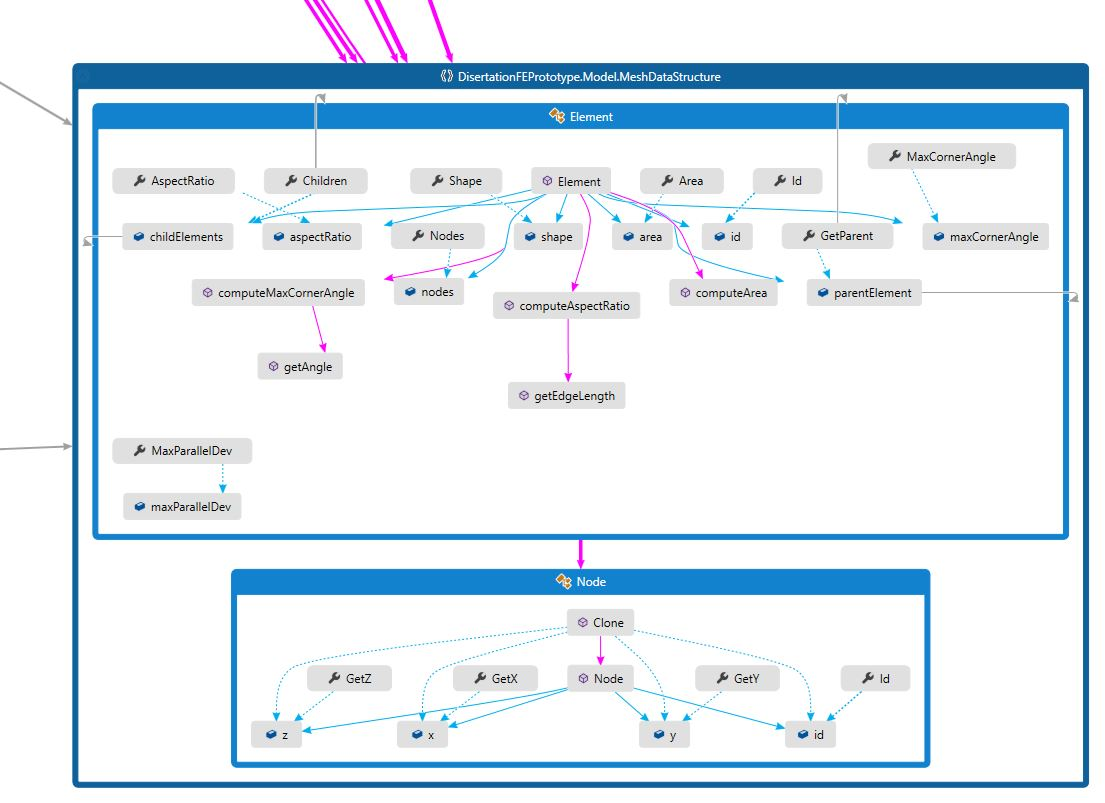
\includegraphics[width=0.9\linewidth]{../Graphics/DissoFEProto-ElemNode.jpg}
  \caption{Element and Node classes}
  \label{fig:sub2}
\end{subfigure}
\label{fig:test}
\end{figure}

\begin{figure}
\centering
\begin{subfigure}{.5\textwidth}
  \centering
  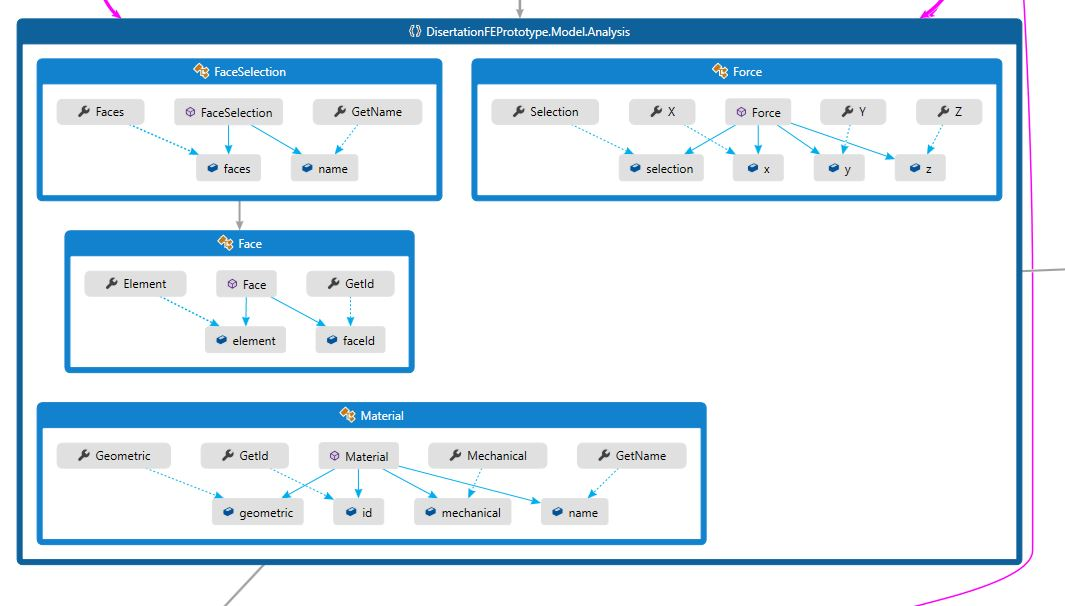
\includegraphics[width=0.9\linewidth]{../Graphics/DissoFEProto-ModelAnalysis.jpg}
  \caption{Model Analysis classes}
  \label{fig:sub1}
\end{subfigure}%
\begin{subfigure}{.5\textwidth}
  \centering
  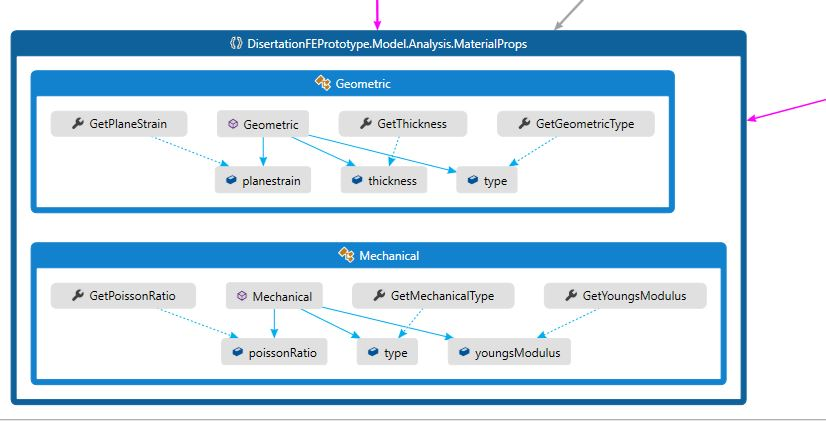
\includegraphics[width=0.9\linewidth]{../Graphics/DissoFEProto-MaterialProps.jpg}
  \caption{Material Property classes}
  \label{fig:sub2}
\end{subfigure}
\label{fig:test}
\caption{Class model to represent .liml file structure used by LISA}
\end{figure}

\noindent
One aspect of the data models design which greatly adds to the systems flexibility is the hierarchical design for representing the various Element types. At the root of this structure is the IElement interface, all new Element types must adhere to this in order for the various refinement methods to request refinement of an element using its class. Implementing the interface are a range of abstract classes such as ``SquareBasedElem" and ``TriangleBasedElem" These classes are designed to contain methods that are generally applicable for calculating metrics and re meshing individual elements where the elements fit this abstract category but their concrete implementation specifies their dimensionality and number of nodes, see Figure 6. This is powerful since computing metrics and performing subdivision for a 3d element is simply a reduction using the code for a 2D element but over every face comprising the 3D one. \\ 

\begin{figure}[h!!]                                                   
  \centerline{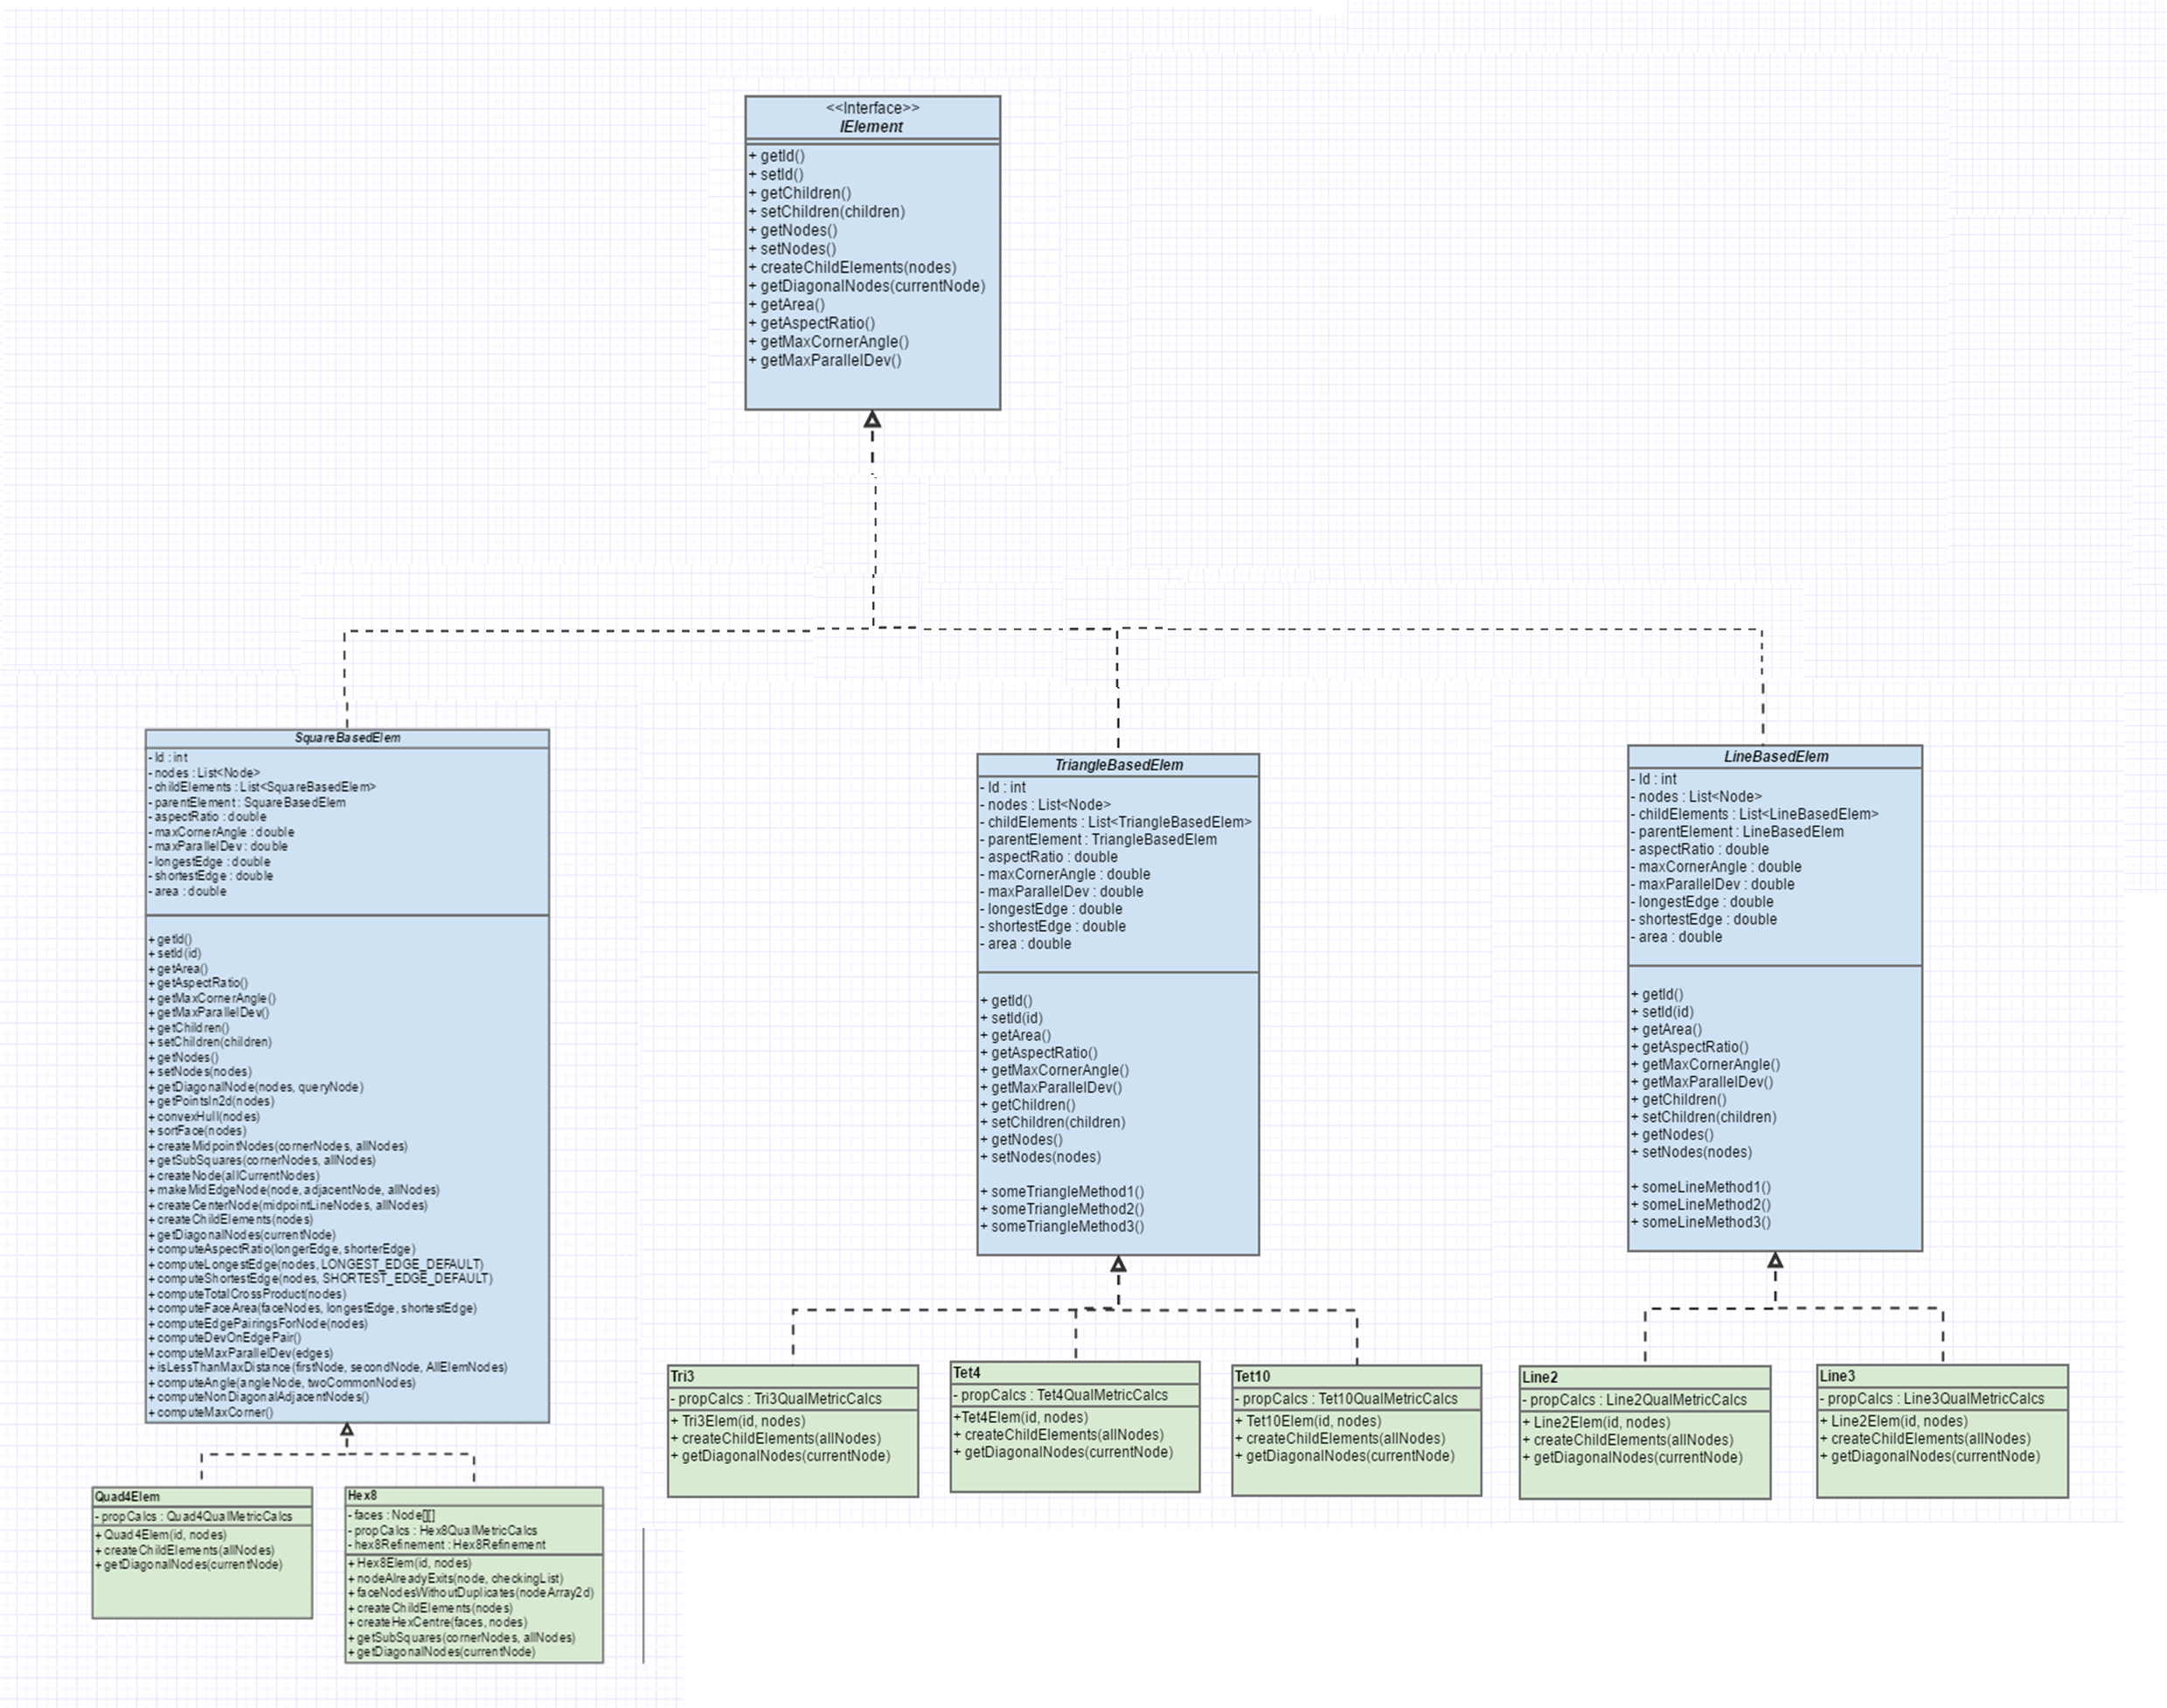
\includegraphics[width=150mm, scale=1]{../Graphics/ElementHigerarchyDiagram2.png}}
  \caption{Class diagram showing the hierarchy of element classification within the data model, due to time limitations I was not able to implement the respective classes for triangle and line based elements, to see image representations of each element type within this class diagram refer to element type appendix}
  \label{fig:h-refinementImp}
\end{figure}


\subsection{Remeshing methods approach}

Delegating refinement of individual elements to their respective classes made it much easier to decouple both the stress and heuristic methods allowing each of them to simply have the task of selecting elements which they considered beneficial to refine before calling the createChildElements() method on that element through the IElement interface. This allowed both of these high level refinement approaches to utilise the same low level functionality thus greatly improving code reuse and simplifying the design such that the high level meshing methods are relatively concise. \\

\noindent
Having reviewed both h-refinement \cite{HandPRefinements} and r-refinement \cite{RRefinement} as techniques for performing element subdivision it was concluded h-refinement was prefferable due to its simplicity and widespread use despite typically being more computationally expensive than r-refinement \cite{HandPRefinements} \cite{RRefinement}. \\ \\ \\ \\ \\

\noindent
Upon finishing subdivision and producing new child elements stored within their parents the refinement process also needed to flatten each tree to produce a new set of model elements. This task involved the deletion of parent elements and therefore needed to be performed by the ``OptimisationManager'' class responsible for combining and executing both refinement methods. \\

\noindent
Having evaluated a variety of approaches from the domains of AI it was concluded that the best approach for delivering a system capable of meeting the requirements and demonstrating effectiveness of a hybrid method would be an implementation of the heuristic expert system described by Dolsak. \\ 

\noindent
One key strength of selecting this approach as the alternative method by which to mesh was clear separation of the underlying AI method from what had to be implemented. This not only meant that focus could be given towards the design, implementation and evaluation of the general purpose system but demonstrated that the meshing procedure can for the most part be interchanged depending on the specific type of finite element analysis. \\ 


\subsection{Input Files}
The system requires three basic input files which should be placed within a directory that is given to the program as a parameter, these are files are:

\begin{itemize}
\item A structural model represented as a .liml file which LISA can solve.
\item An initial stress data file generated manually so the system has a starting point.
\item A JSON file containing important edges and associated meta data as identified by an engineer looking at the model.
\end{itemize}

An example of the content and format for each of these input files can be seen in Appendix B



\subsubsection{Combining methods}
Since each refinement method performed a discrete amount of subdivision every time it was called it made sense when developing a hybrid approach to simply enumerate the possible combinations for how much each method could be applied each iteration resulting in a set of two valued tuples up to some value :

\[ \left\{ (a, b) \,\middle|\, \, a,b \in \mathbb{N}\, \, a,b < k \right\} \]


\colorbox{yellow}{not sure if anyone actually cares about multithreading}

\noindent
Each tuple could then be considered one weighting configuration for combining the two methods and could be executed independent of the others to obtain a set of results for that weighting. Consequently it was possible to improve performance when conducting multiple evaluations through parallelism of the different weighting configurations as experiments onto independent threads. When started each thread creates its own directory which it copies the three input files to and runs for its designating weighting configuration. 




\section{Software Implementation}
The following subsections detail the implementation of the final software solution that has been written to meet the objectives posed at the beginning of this dissertation.

\subsection{Third Party FE Application}
In order to demonstrate the potential feasibility of the hybrid approach it was first important to obtain a finite element solver which could be given a FE model containing data about forces, materials and the mesh structure and then execute the model pro grammatically so as to obtain stress results. \\ 

\noindent
A multitude of commercial FE tools exist with there being a wide variety in both the complexity and cost associated with each tool. 
Finite element software is typically very expensive due to its high development cost and small customer base. Tools used within industry such as ANSYS typically require a great deal of time in order to become proficient in their usage and can cost in excess of five thousand pounds a year for a single licence \cite{AnsysCost}. It was therefore important to find a tool which was both affordable while also powerful enough to demonstrate a working prototype of the re meshing method.
 
\subsection{LISA}
After reviewing several FE applications used within industry in addition to a variety of less well known ones used within academia and by hobbyists LISA  was selected as the solver application for which to implement  the systems prototypes. \\ 

\noindent
\textbf{Strengths: }LISA as a FE tool which allows the user to run models of up to 1300 element for free; This was beneficial in allowing me to experiment with the software and gauge the feasibility of my projects concept before requiring a full version. Once at a stage in the project where each problem had been solved for small models containing less than 1300 elements an academic licence for the software was purchased for the projects use. \\

\noindent
LISA also provides a GUI which allows visual inspection of the model and its mesh; This is particularly useful for observing the output of the meshing algorithms which can often provide a human with a much better understanding of how the method has performed and whether or not there are obvious bugs. in the implementation of the meshing procedures \\ 

\noindent
\textbf{Weaknesses: } Due to LISA’s simplicity it does not come with an extensive API allowing for easy programmatic use of its inbuilt features, however it is still possible to interface with LISA through less direct means \cite{LISAManual}. LISA models are stored in .liml files which use XML as a meta mark-up format. The model files contain all the information about the model including the materials used as well as loads and constraints and of course the mesh. It is therefore possible to manipulate a .liml file having parsed its contents before writing a new version of the file which LISA can be called to solve. In order to more easily alter the model it made sense to write a wrapper  for the .liml files to abstract the manipulation of their content.

\subsection{Languages and platforms}
The final system has been written entirely using the C\# programming language (version 5.0) with Visual Studio 2015 as the development environment on a Windows 10 system. C\# is an application development language built on the .NET framework. Although any number of programming languages could have been used to implement the solution C\# offered a good compromise for developing a system with both structural rigidity through static typing and object orientation in addition to functionality to allow for rapid prototyping. C\# does this well through use of LINQ, a part of the standard library that provides a large number of higher order functions which allow for operations to be performed over any data structure that implements the built in IEnumerable interface. Given that much of the code within the project performs the same operation on collections of nodes and elements stored in Lists arrays and dictionaries which all implement IEnumerable the ability to write much of the project using this capability dramatically reduced the number of errors encountered and increased development speed.


\subsection{Implementation Methodology}
Due to the size of the software, which is now in excess of 14000 lines of code it was important to work systematically to continuously drive the project in the right direction and avoid the introduction of unnecessary complexity. This was achieved through regular reviewal and refactoring which dramatically helped to reduced the amount of bugs introduced. \\

\noindent
For the duration of the project the spiral methodology was adhered to. This enforced multiple deliverable stages that were concluded with a supervisor meeting every one or two weeks. Adopting the spiral methodology also provided flexibility regarding the order in which tasks were able to take place outside of a spiral iteration. This was necessary when conducing a research driven project where direction of work for subsequent development iterations was largely driven by the  findings of the work in the previous ones. \\

\noindent
Tasks were chosen every week for the project, the number of tasks and their complexity was determined using a combination of factors including their complexity, the criticality of the task e.g. Did it need to be completed for other important tasks to be started and the time available to me as the individual undertaking the project (More tasks typically performed on weeks when less work was due for other modules.

\subsection{Implementation of Subsystems}
This section describes the implementation details of the various different subsystems which combine to form the overall solution.

\subsubsection{Re-meshing using hierarchical refinement}
After reviewing both h-refinement \cite{HandPRefinements} and r-refinement \cite{RRefinement} it was concluded h-refinement would be best the best approach to adopt due to its simplicity and more widespread use \cite{HandPRefinements} despite the fact that the mesh is usually more computationally expensive than it would have been if it was created using r-refinement \cite{RRefinement}\\ 

\noindent
Elements within traditional FEA can typically be classified as either triangle or square based elements, each of these provide different strengths and weaknesses when required to mesh and solve models. Within industry triangular elements are typically preferable since it is always possible to generate an initial triangular mesh from any arbitrary CAD geometry algorithmically. This is done by simply making smaller triangles until all gaps along the edge of the geometry are filled \cite{DelaunyTriangles}. The same cannot always be said  when meshing using square elements. For proof of the solutions concept however it was concluded that square based elements were preferable to triangular ones with since the steps required for a basic refinement are much simpler, just take the corners of an element that already exists, add their x, y and z components before dividing each component by two to achieve the coordinate for a node which is halfway between the two. \\ 

\noindent
In addition to refinement it is also significantly easier to define edges which the ILP rules can be applied to when edges naturally form within a structure through a chain of nodes along the edges of square elements.

%The process of re meshing square based elements 

\noindent
Unfortunately Triangular meshes also generally incur a higher computational cost than an equivalent square element mesh due to added complexity of performing the calculations required to remesh in addition to requiring more elements over a given area to achieve the same accuracy. \\

\noindent
From an implementation standpoint writing a square based remeshing algorithm is also substantially easier as given an initial mesh made just of square elements the only task is to repeatedly divide each element into four sub elements, by contrast methods uses to re mesh triangular meshes vary greatly are typically more complex and have corresponding initial meshes that are harder to generate manually by human operators \cite{HandMeshing}. \\ 

\subsection{Fast node lookup and update of nodes}
A key requirement for the design of the data model generated by the hierarchical re meshing process was the need to perform fast lookup of nodes already present in the mesh. Lookup is important within the meshing methods as a means of checking whether a node that is about to be created already exists within the model, in the event that no such node already exists a new one can be created however if it does then instead of creating a new node the node that already exists needs to be connected to a node in an adjacent element that is currently being refined. If nodes are not linked correctly form correct elements the physics solver is unable to assume the stress moves through one element to another despite both having nodes at the same coordinates, this results in inaccurate output or potentially an error being thrown by LISA. \\ 

\noindent
This issue arose as a result of partly as a result of the systems design, as previously mentioned subdivision for every individual element is the responsibility of that element which from a software engineering perspective is very good since it means the low level meshing process for each different type of element could be written within that elements class. This avoids the need for much heavier generalised refinement classes that would have needed to know how to perform the meshing for all elements in the model at once and for each of the different potential element types. A consequence of this was despite every Element being capable of meshing itself perfectly adjacent elements that also requiring refinement needed the ability to reconnect the new nodes along their edges to those that had created by the adjacent element. \colorbox{yellow}{This can be seen below in figure x} \\ 


\begin{figure}[!h]
  \centerline{\includegraphics[width=100mm , scale=1]{../Graphics/nodeLinking.png}}
  \caption{The need for an element to check for existing adjacent nodes when subdividing itself during refinement,\\ \\
  	Orange Nodes - An original node for one or more elements \\
	Red Nodes - new nodes made by Elem A \\
	Purple Nodes - new nodes made by Elem B \\
  }
  \label{fig:h-refinementImp}
\end{figure}


\noindent
The solution to this problem was to store all the nodes in the mesh model within a C\# dictionary structure a reference to which is passed to each element within the model. The dictionary can be indexed using a Tuple of the x, y and z coordinates for the new potential element which will either return a node already at that location or indicate that no such node exists, in which case that element is then responsible for creating the node as its first instance. Dictionaries in C\# represent a generalised instance of a hash table ensuring that lookup and insert are both constant time on average.


\subsection{Sorting Element Nodes in 3d space using convex hull Algorithm}
A significant issue encountered when working with LISA on the project was an interface requirement specified by LISA requiring nodes for each type of element to be sorted in a specific geometric order. The general rule for node ordering within LISA is to order the nodes as a perimeter around an element in 3d space without paths between nodes crossing one another internal to the element. When first addressing this problem for simple models using elements of Quad4 type the obvious approach was to think of a simple quadrilateral resembling a square, write an algorithm to handle that as a base case before considering a more complex case. The resulting approach was the following approach:

%do pseudo code for initial approach here
\noindent
This approach was sufficient for the vast majority of elements within the different models, however as model complexity increased multiple iterations of the heuristics resulted in increasingly distorted element shapes, resulting in rejection of elements with incorrectly sorted nodes by LISA. \\
 
\noindent
In order to resolve this issue I needed to research and apply a convex hull algorithm to this problem. The subsequent solution was the following: \\ 

%algo 1

\noindent
Despite the existence of algorithms for generating a convex hull in three dimensions due to the small number of points it made sense to assess the effectiveness of a 2d method first before committing and assess the effectiveness of that for resolving my problem. In order to do this I simply took my Quad4 elements and flattened them to a 2d representation by calculating the maximum delta between the greatest and smallest value on each axis and eliminating the axis with the smallest delta. This proved successful, when applied to the model this successfully removed incorrect ordering from elements that had been particularly skewed. \\ 
	
%algo 2

\noindent
This method has O(n log n) time complexity however due to the size of n being 4 in all cases the complexity of sorting an individual element is constant, with the overall complexity of sorting all elements in the model being O(n) where n is the number of elements.


\subsection{Stress Based Refinement}
To focus meshing in areas of high stress each iteration needed to parse the results file from the previous iterations execution of LISA. LISA result files are in csv format by default and contain the displacements and stresses associated with each node within the model once it has been solved.

Once the data in the output file has been parsed meshing can be conducted for high stress areas by averaging the stresses across the whole model and then cross referencing the node Ids in the results which have stresses above the average against the main data model allows a list of elements that can be instructed to refine themselves.


\subsection{Rule Based Refinement}
Each rule is represented as a function within the implementation, this closely resembles the format presented by Dolsak \cite{DolsakPaper91, DolsakPaper94, appOfILPToFEMeshDesign} \cite{ConsultRuleIntelltSystemFE}. Each of the rules resides within the ``RuleManager" class and takes a number of the defined edges as parameters. Each rule then checks the properties of a particular edge against properties which have been identified through the ILP learning mechanism as being important when the model executes. In cases where the rules accept more than one edge as an argument the rule is applied to all combinations of possible input edges. If a rule detects a relationship in the model the edge is assigned a criticality rating as defined by the rule, the value is then used by the meshing procedure to determine how many times it should repeatedly re mesh the elements along that edge. \\ 
 
The properties that can exist between two edges when compared are the following:
\begin{itemize}
\item Edges opposite one another - the edges run alongside one another closely
\item Edges posses the same form - 
%finish this

\item Edges are considered the same - to meet this requirement both edges must be almost the same length, opposite one another and posses the same form.

\end{itemize}


\subsection{Mesh Quality Assessment}
Dittmers rules for computing the quality of both individual elements and the entire mesh are built into their own ``MeshQualtyAssessments" and ``ElementQualityMetrics" classes, the latter of which is encapsulated within an element object, like with refinement this allows each element to assess its own quality removing the need for additional utility classes containing static methods. \\

%not sure about the last sentence here
Since each element is initialised with the nodes that comprise it, it is also possible to derive all the geometric characteristics and thus its quality metrics upon its initialisation. This allows the metrics for each node to also be calculated upon its initialisation removing the risk of elements returning null when asked for them.

%Upon evaluation of the project and concluding that effectiveness of the heuristic relied upon overlap of the %heuristically mesh area with areas of high stress

\subsection{Implementation Issues}
Implementation of the design was not without its difficulties, many of which arising as a consequence of unforeseeable complications when implementing the well understood theoretical aspects.


%Think about putting this under evaluation or removing it instead
\subsubsection{Attempts to Automatically Define edges within models}
As discussed under evaluation one of the main issues faced was identifying where the system behaved poorly through weakness in the methods or poor design and implementation as opposed to poor output generated as a consequence of poor input by the operator. In order to avoid this issue it was desirable to try and remove user intervention besides the configuration of the initial model. The obvious way by which to do this was automatic identification of interesting edges within the model. A crucial property which made this approach appear promising is the fact that it is known that edge importance directly correlates with the size of the edge and how much force is applied near it, since both this information exists within the data model it should be possible to identify edges from it and generate them automatically for Dolsaks rules to process.  \\


\noindent
In practice there are multiple complications surrounding this, several of these arise from ambiguity in Dolsaks paper regarding what constitutes a an edge which is for example "long" or "important". As a result edges are only able to be defined to the extent that a user has confidence in their understanding of these concepts. \\ 


Having considered a method using these properties of the mesh several days were then spent attempting to implement it with poor success achieved.


\section{Evaluation of Project}
Evaluation of the project consisted of multiple stages ranging from verification of the functional requirements through simple black box testing to evaluation of refined mesh quality using methods provided by Dittmer \cite{DittmerMeshQualityMet}. 

\subsection{Validation Against Functional Requirements}
In order to validate the system against many of the functional requirements the system had to be run on a number of basic models with different input configurations. Having done this the results clearly demonstrate the system's ability to evaluate the quality of meshes using multiple refinement processes based on the stresses present within the structure and the specification of edges by a user. \\ 

\subsection{Validation of Software Quality}
\noindent
In the case of quality for the system's design and documentation evidence is provided in, (see appendices C, G and H)  to the requirements specified with the project submission containing detailed documentation in the form of a Deoxygen guide which shows the use of object oriented and functional software design as seen within the codebase. General applicability of functionality has also been demonstrated through evaluation using a variety of models and conditions when performing simulations.

\subsection{Unit Testing}
Holistic evaluation provided evidence of the overall system's effectiveness. Verification of individual components created trust in the accuracy of the results produced. Unit testing was also conducted from within Visual Studio (VS) using the NUnit framework and structured as a separate VS project. This guaranteed that the system was not able to interact with the tests and that testing was conducted through the class and function interfaces provided by the implemented solution. Tests were also grouped into classes with each test class corresponding approximately to one class within the system. Each test class then contains a number of test functions each of which performing the asserts necessary to deem its associated function as correct. This layout provided clear traceability from each item of functionality to its associated test making assessment of the test coverage much easier. Appendix B shows the visual studio test explorer containing the various tests. \\


\subsection{Software Quality and Management}
The software was developed using industry best practice including the use of appropriate variable naming, loose coupling of classes, use of abstractions and descriptive error messages which make the software easier to read and debug for any potential future developers. An effective version control strategy was also adopted by backing up all software to Github daily. \\

\noindent
Visual Studio also enabled calculation of various software quality metrics for the code base automatically. This made selecting parts of the codebase for refactoring much easier. Upon completion of the project the average maintainability index \cite{VisualStudioMaintainIndex} across all modules was 75 with the lowest score for any high level module being 60 and the highest 92. According to the Microsoft Developer Network (MSDN) website code with an index of between 0 and 9 indicates low maintainability, 10 to 19 indicates moderately maintainable and 20 to 100 high maintainability. \\ 

\subsection{Documentation}
The process of continuously writing descriptive documentation was important to the success of the project and was treated as an integral part of meeting the goals of the projects development methodology which aimed to reduce the systems complexity and improve readability. Through the writing Doc comments corresponding to every function within the codebase it was possible to generate documentation files automatically through use of the tool Doxygen. This allows anyone with the solution to view descriptions of each of its functions either in the codebase or alternatively through the manual produced automatically by Doxygen, for example see appendix. \\ 

 

\subsection{Evaluation Of Hybrids and Individual Methods of Refinement}
%To demonstrate the systems applicability to a variety of real engineering problems demanded the creation of several models resembling basic equivalents of real structures that are often analysed by FE methods.

%As a system designed to facilitate analysis of hybrid meshing techniques the ability to conduct detailed evaluation for a set of hybrids over multiple simulations demonstrates successful generality. \\

In order to validate the different methods of refinement it was important to carefully design tests for the system which would fairly measure its ability to compare a range of hybrid methods capable of performing meshing. \\ 

\noindent
Firstly it was important to test the various methods individually for at least one model in order to verify that each of the methods performs as expected, this is a key step in order to have trust in the results subsequently produced by the hybrids. When evaluating the hybrids the system also needed to be evaluated for several different FE models with varying simulation conditions. This demonstrates consistency in the results and the systems ability to work for a range of different model inputs. \\

\noindent
Hybrid performance evaluation should consider both good and potentially bad user input.  

\noindent
Three models were created in total for evaluation, with each of the models being a general simplification of a more complex model that could be expected within an industrial engineering setting. They model a suspension bridge, a part of a paper mill and a section of a generic cylinder. These models were developed specifically for the project although the paper mill and cylinder were based on two models used by Dolsak in order to train the ILP method when generating the rule set. Each model has a manually constructed low fidelity mesh built using LISA's graphical user interface. The models also have a set of forces applied to them which are required so that stress is induced within the simulation. Constraints are also assigned to surfaces as described under section 2.1. The results for the two models not analysed in this section (the cylinder and paper mill disk) can be found in appendices K and L. \\ 


\noindent
\textbf{Different Quality Edge Specifications: } Validation of edge specifications to reflect real world conditions was necessary, see 6.4 for heuristic edge specifications. Since the users specify the edges that determine the meshing focus they directly affect the final result of the process, it is therefore important to consider the results produced by the system for a variety of different potential users. The effects of good and bad edge specifications can be observed both in execution times for the simulations and in the system's ability to mesh accurately where required as seen in figure 15 and the mesh structure in appendix J. \\ 

\noindent
Since the three models were very different it was not possible to objectively compare the edge specifications for each of them. a basic criteria was therefore developed so that comparisons could be drawn. For each model four sets of edges were consequently constructed and given classifications of ``Best'', ``Good'', ``Ok'' and ``Poor'' With the following as general guidelines for defining each set: \\

\noindent
\textbf{Best: } Approximately five edges specified directly over or adjacent to those areas of known high stress within the model - input potentially generated by a user with a high degree of expertise in evaluating the specific type of structure. \\ 

\noindent
\textbf{Good: } Approximately three edges over or close to areas of high stress within the model - input potentially generated by a user with a high degree of general FE experience although potentially not specific to that type of structure. \\ 

\noindent
\textbf{Ok: } Three to five edges some near high stress and other not - representing a user with some experience but by no means an expert. \\ 

\noindent
\textbf{Poor: } Three to five edges none of which are close to areas of high stress - representing input as would be generated by an inexperienced user new to FE stress analysis. \\ 

\noindent
Not being a mechanical engineer it was necessary to find a way of defining what `Best' and `Good' looked like. To do this the traditional stress based refinement approach was run on each model to establish where high stress areas exist before using this to define a series of edge specifications of varying quality. Consequently it is only possible to objectively judge each of the different sets on the basis of the results they produce. These results would have had greater validity if time had allowed input from a range of practicing mechanical engineers. \\

\noindent
 
\subsubsection{Metrics Selections}
Due to the complex nature of finite element models there are a number of potential methods that can be used to evaluate the effectiveness of my approach. The metrics I eventually selected along with a description of what they indicate and why this was important to conclude the systems ability to meet its objectives is detailed below. \\ 

\noindent
\textbf{Average Maximum Internal Corner Angle: } This metric was cited by Dittmer \cite{DittmerMeshQualityMet}as one of the most consistent indicators by which to evaluate the quality of a mesh with gradual deviation from the optimum indicating a degradation in quality and the meshing processes inability to maintain quality and consequently ensure accuracy of subsequent results. Figure 3 show types of distortion, such as skewing, which can be detected by measuring the internal corner angle. \\ 

\noindent
\textbf{Execution Times: } Since it is important for all methods to run in a reasonable amount of time, measuring the increase in runtime with additional iterations provided a good indication of how costly each approach became and whether there were any points at which refined meshing became significantly more expensive. Comparing the execution times for the different approaches also indicates how much work each method is doing per iteration allowing the hybrids to be balanced, see section 5.8. \\


\noindent
\textbf{Average Stress Revealed for Each Iteration: } In order to measure the different methods ability to reveal stress over time the average stress across all the elements throughout the model is an effective metric to use. An increase in the average occurs as a result of more elements being placed on those areas of high stress and decrease occurring with creation of elements over areas of lower stress. Since this metric is a measurement of stress which is force over a given area stress is essentially a measure of pressure and as such the unit of measurement used is pascals. To simplify evaluation so as to take into account the different edge specifications the hybrid data below is based on the average values obtained for the heuristics when running all of the edge sets for the different models. \\ 


\subsubsection{Evaluation of Bridge Structure}
The suspension bridge model (see figure 19) consists of 196 elements of quad4 type and 212 nodes which can be considered coarse given the size of the structure. Four constraint points were specified at the base of each supporting column and strong forces were applied across the structure along the negative x axis. \\

\noindent
\textbf{Evaluating Individual Refinement Methods: } 
\noindent
 An important part of validating the proposed hybrid approach was to first evaluate each of the refinement methods individually and observe their performance. This then informs the weighting applied to each method to avoid either method dominating the results of the hybrid approach. To test the individual approaches effectiveness they were evaluated against the performance metrics defined in section 7.6.1 (i.e. time required to refine per iteration and average maximum internal element angle). The results of these validation tests are shown in figures 15 and 16. From these graphs it can be concluded that no individual method reduces the mesh quality and that both the individual methods spend approximately the same amount of time performing refinement per solve iteration meaning neither is overly favoured by a hybrid approach.
  

\noindent
 \\

% show angle and runtime



\begin{figure}[H]
  \centerline{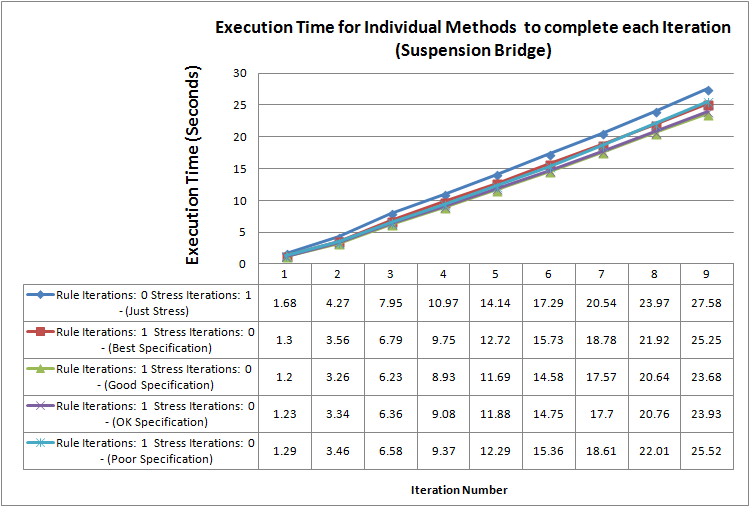
\includegraphics[width=110mm, scale=1]{../Graphics/FinalReportGraphs/ExecutionTimeIndividualMethodsSuspensionBridge.png}}
  \caption{Time taken to complete each iteration using the different methods}
  \label{fig:sub1}
\end{figure}  





 
\noindent
The maximum internal corner angles can be seen as improving linearly over time although with the greatest rate of improvement occurring during the first few iterations for each method before the average for the mesh approaches the optimum, which for elements of type Quad4 is 90 degrees. This means in general the refinement methods reduce skew present within the model through the creation of new elements and the calculated stress retains its accuracy. 

%This indicates that the refinement methods tend to reduce element skew within the mesh by effectively smoothing the mesh. This suggests that the results produced by the solver can be assumed to be at least if not more accurate after the mesh has been refined than before. This trend also extends to the other two evaluation models suggesting that the underlying subdivision process does not generate meshes that compromise the calculation of stress values for any input mesh.


\begin{figure}[H]
  \centerline{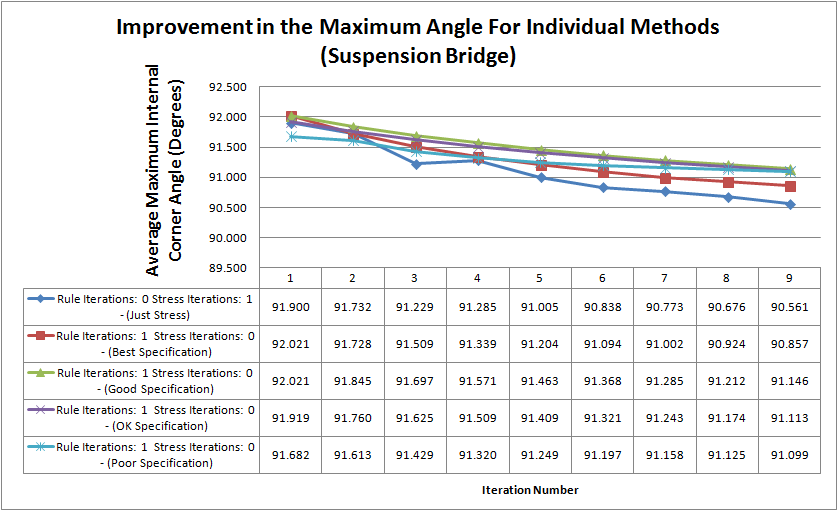
\includegraphics[width=110mm, scale=1]{../Graphics/FinalReportGraphs/AngleImprovementIndividualMethodsSuspensionBridge.png}}
  \caption{Approaching the ideal quad4 geometry for simulation data accuracy of 90 degrees using refinement with each of the different methods}
  \label{fig:sub1}
\end{figure}  

\noindent
%A key realisation having calculated the average maximum angles for the different methods was although Dittmers metrics helped to indicates that the results produced by the solver are accurate they do not actually demonstrate one refinement methods ability to mesh in more desirable areas than another while retaining a lower computational overhead through creation of fewer elements, an alternative metric was clearly needed in order to show this. A simple solution which proved highly effective was simply to calculate the average stress across all nodes. By calculating the average each method effectively achieved a high score for placing few elements directly over the high stress area while avoiding element creation over lower stress areas that would reduce the average.\\ 


\noindent
 

\noindent
\textbf{Evaluating Hybrid Refinement Methods: }
\noindent
When used on their own the heuristics (rules) based approach to FEM refinement revealed greater stresses than the traditional stress based approach. This is evidenced by figure 17 where after 6 iterations a heuristic approach had revealed stress levels up to the value of 6.3E+31 pascals whilst the traditional stress based approach revealed up to 4.5E+20 pascals. It can be concluded that there is demonstrative value in using a heuristic (rules) based approach regardless of whether used on its own or as part of a hybrid refinement strategy. \\ 

\noindent
Having completed analysis for each of the individual methods tests were run using hybrid strategies for each of the models. This produced results that indicate rapid overall improvement with regards to finding stress as can be seen below in figure 17 below. The improvement can be seen during the first few iterations in figure 18 before achieving a plateau.  The accuracy of the results were initially questioned with the values being extremely high, however Re-execution of the model with varying configurations including varying force and alternative constraints resulted in minimal differences. Conducting additional research revealed that this is not in fact an uncommon property of stress gradients within FE models \cite{StressConcerntration} as the calculated values for stress stress will trend towards infinity at points of serious weakness within a design when a high force is exerted and the stress is able to concentrate at particular points. A real structure would not be able to enduring stresses of these magnitudes and would break at these points of stress concentration before the stress calculated by the solver could actually occur.  Figure 19 below shows the bridge model undergoing relatively high stress at various points across the model but with rapid increase at specific points where structures join one another (highly focused red patches in 19b). \\


\textbf{\begin{figure}[H]
  \centerline{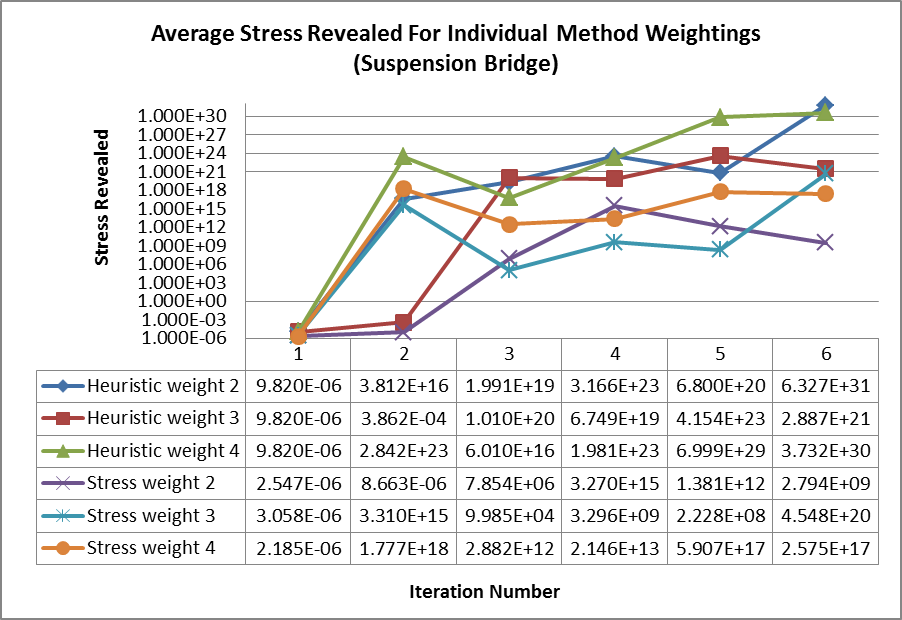
\includegraphics[width=110mm, scale=1]{../Graphics/Graphs/AverageStressesBridge/AverageStressRevealedForIndividualMethodWeightings.png}}
  \caption{Average stress revealed with different weightings for the individual methods}
  \label{fig:sub1}
\end{figure}}


\textbf{\begin{figure}[H]
  \centerline{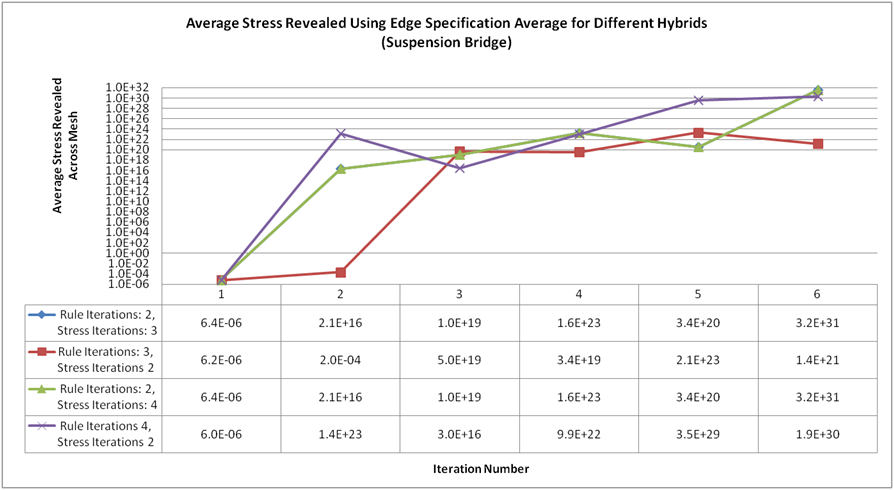
\includegraphics[width=110mm, scale=1]{../Graphics/FinalReportGraphs/AverageStressRevealedSuspensionBridge.png}}
  \caption{Average stress revealed using multiple iterations of the different hybrid methods over time}
  \label{fig:sub1}
\end{figure}}


\noindent


\noindent
Figure 19 indicates some unpredictability in the hybrid results i.e. when combining the individual methods. For example hybrid (3, 2) shows poor performance until iteration three while the other hybrid approaches, show similar accuracy to the individual methods. All the hybrid methods show greater consistency of results after iteration 3. \\ 

\noindent
When combining the heuristic and stress based approaches together to form a hybrid approach the level of stress found and the speed at which it was found was no worse than using the heuristics approach on its own. This is evidenced by comparing data from figure 19 (hybrid plots) against figure 17 (individual plots) i.e. after 6 iterations the hybrid approach had found stresses of value 3.163E+31 pascals against a figure of 6.32E+31 pascals for individual plots. \\ 

\noindent
From this observation it can be concluded that the influence of the heuristics on the overall hybrid approach is much greater than anticipated. Even when this affect is compensated for by using a hybrid strategy which heavily weights in favour of the stress approach (e.g. where heuristic rules weighting = 2, stress weighting = 4) the average stress after 6 iterations remains similar to a rules only approach. This suggests the need for further work to identify why this is occurring and then feed this back into the weightings for future development. \\

\noindent
Having run the model with the hybrids the coloured stress gradients across each structure can be inspected by an engineer, see figure 19 and appendices J below. LISA assigns colours to different ranges of stress based on the range of values within the model. In the majority of cases red areas represent those areas of highest stress followed by orange, yellow, green, light blue and eventually dark blue.  \\ 


%say something about how actually you want a bit of distribution
%\noindent
%Comparing the amount of improvement performed by both the stress and heuristic refinement processes with varying weightings that in general heuristics performed better than stress refinement although interestingly more weighting did not necessarily correlate to better results as can be be seen with heuristic weighting of two doing a better job than weighting four in the final iteration. \\

%../Graphics/BridgeCrossLoadingStress/bridgeStressBasic.png
\begin{figure}[H]
\centering
\begin{subfigure}{.5\textwidth}
  \centering
  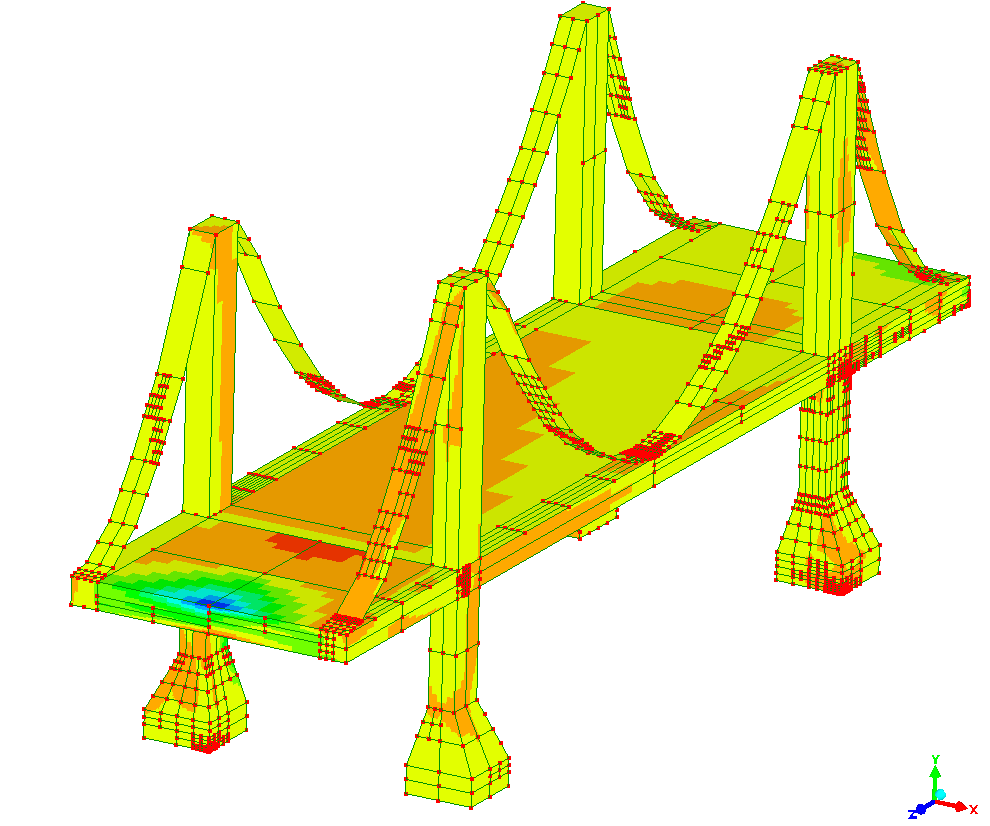
\includegraphics[width=0.9\linewidth]{../Graphics/BridgeCrossLoadingStress/Hybrid-best-3-2.png}
  \caption{Stress Revealed through the initial highly coarse bridge mesh without running any iterations for either method}
  \label{fig:sub1}
\end{subfigure}%
\begin{subfigure}{.5\textwidth}
  \centering
  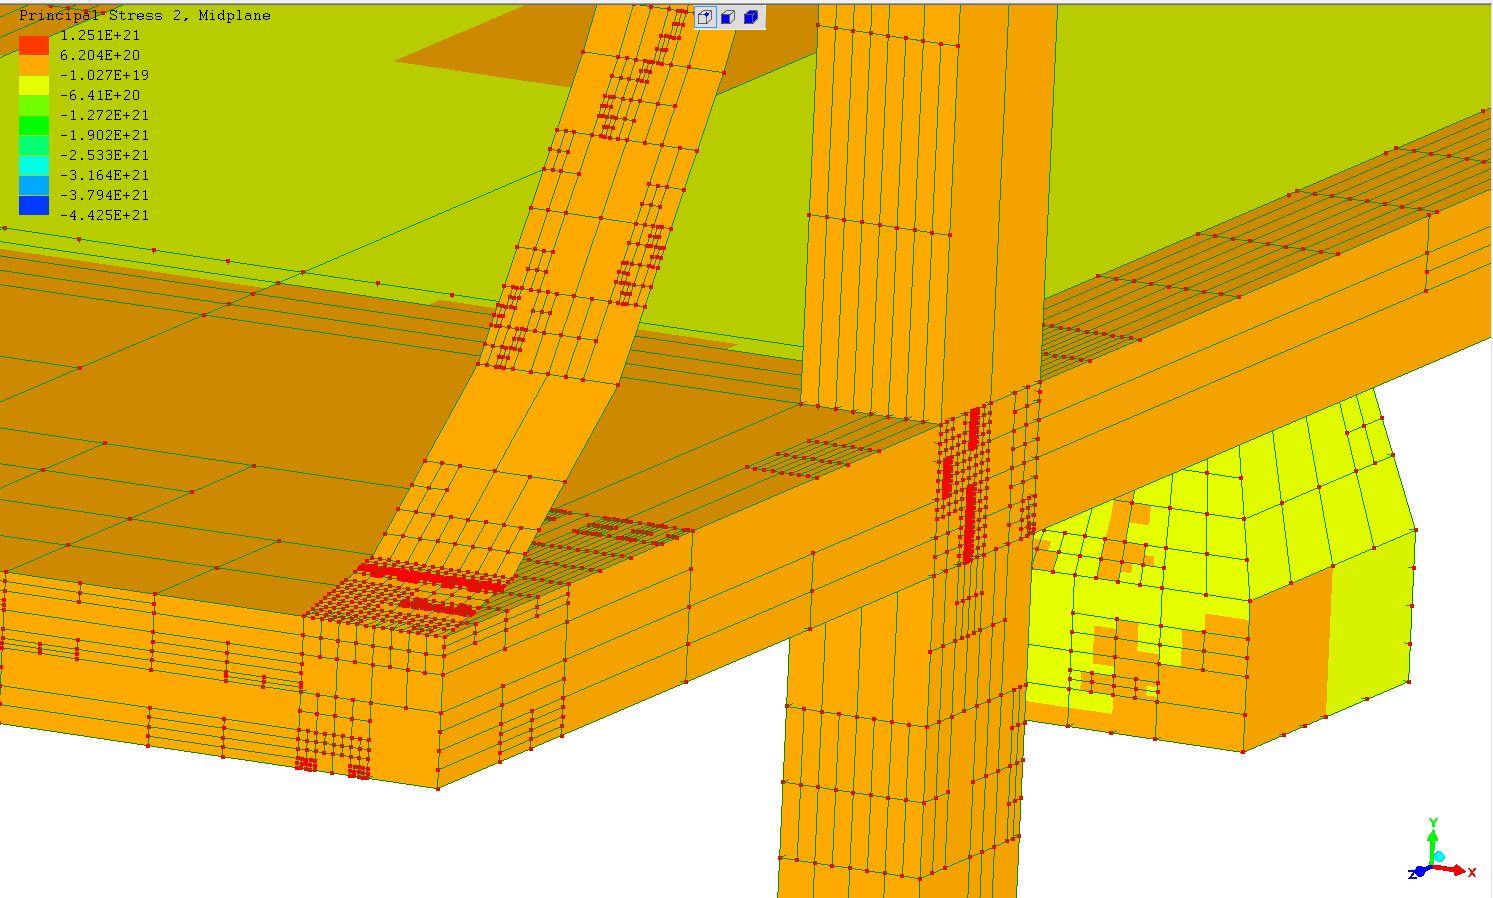
\includegraphics[width=0.9\linewidth]{../Graphics/BridgeCrossLoadingStress/BridgeCrossLoadingStress6-3-2.png}
  \caption{Meshing highly concentrated in those areas of the structure where the stress converges}
  \label{fig:sub2}
\end{subfigure}
\label{fig:test}
  \caption{Stress revealed within model after just 4 iterations with a heuristic stress method weighting of 3-2, edge heuristics also considered good in this case}
 \end{figure}



\noindent
In addition to the data summarised in this section of the report additional data collected for the various hybrid approaches applied to two other models is summarised in Appendices K and L. These results show how the hybrid approaches perform against the performance metrics identified in section 7.6.1 and provide reassurance that whilst the hybrid method cannot conclusively be demonstrated to calculate stress quicker than traditional methods the quality of the output (as measured by the performance metric) is as good as any other method used. 


\subsection{Strengths and Weaknesses}
The resulting system successfully satisfied both the functional and non functional requirements in addition to providing insights into the possibilities of a hybrid technique for effective finite element meshing, something that was optimistic at the start of the project but highly desirable. The project was well managed with all of the objectives being delivered as per the initial time plan, see appendix M. Quality was also maintained throughout the project by the application of good software engineering practice. \\

\noindent
The adoption of a modular architecture was a great great strength of the system allowing for a huge amount amount of potential extendability in the future and simplifying the ease with which both the individual methods could be combined to form new hybrid approaches. Although little focus has so far been given to the system's usability it could be developed and distributed as a public tool for experimentation with hybrid meshing with limited additional effort. Another highly flexible aspect is the system's ability to accept any heuristic definition in terms of edges within a mesh structure. Theoretically this means the final system is also capable of using the same types of edge specifications for any type of FE analysis such as fluid flow or heat transfer given a corresponding rule set to inform the refinement of the mesh. \\


\noindent
A downside of the current design is the need for the user to manually specify the edges by manually entering data into the JSON input file which is both time consuming and prone to error despite the relatively small size of the models analysed in this dissertation. Comparing the size of these with those used in industry it is clear that this process is simply not practical for engineers conducting large scale FE analysis. To address this better tools are required that will allow engineers to automatically generate edge specifications quickly, most likely through some GUI or a bespoke high level language capable of combining knowledge about the mesh structure and different types of edges to generate specific rules. Again this is beyond the scope of the project and would likely be a dissertation in its own right. \\


\noindent
Although the system had a strong subsystem and class level architecture many of its weaknesses could be attributed to needing to prioritise the ability to perform rapid prototyping over efficient implementation of the various algorithms and methods described in this dissertation. Much of this a consequence of overusing the functional programming capabilities within the C\# LINQ library. Widespread adoption of functional programming practices was stated as a desirable aspect of the final system implementation within the non-functional requirements in order to simplify the design and reduce unnecessary state, see appendix A. This was largely adhered to with significant use of lambda and higher order functions throughout the codebase. However, in the later stages of the project it became apparent that in many cases reliance on these features over more traditional programming constructs such as loops and conditions resulted in reduced readability of the code and a potential reduction in speed for implementations of the algorithms described in this dissertation.


%%%%%%%%%%%%%%%%%%%%%%%%%%%%%%%%%%%%%%%%%%%%%%%%%%%%%%%%%%%%%%%%%%%%%%%%%%%%%%%%%%%%%%%%%%%%%%%%%%%%%%%%%%%%%%%%%%%%%%%%%%%%%%%%%%%%
\section{Further Work}
This section details some areas which given additional time would be investigated, if not implemented. Each of these areas would hopefully provide some benefit in assisting to further demonstrate the possibilities of hybrid methods.

\subsection{Gathering Feedback From Experienced Engineers}
Approaching the end of the project it became clear that in order to better identify the systems strengths and weaknesses would require additional user testing by engineers who have experience conducting this type of analysis. Feedback from engineers with applied industrial experience along with that of academics would have allowed for a more conclusive analysis of the system and its ability to work across a greater number of general case scenarios. No user feedback was obtained within the duration of the project as a result of time constraints and the complexity inherent in simply implementing and validating the project for a selection of basic models. As such even if time had been available the ethical clearance required to collect user feedback at the start would need to have been acquired.


\subsection{Improving Usability Through A Web Interface}

\noindent
Lack of straightforward portability for the system was one factor that would have made it difficult to get feedback from industry, an alternative approach would be to develop a web interface so as to allow users to easily interact with the system externally. This approach would allow engineers to submit feedback digitally which could then be aggregated from a much greater range of users separated geographically. \\\ 

%Instead by facilitating interaction with the system by means of a web interface the engineers would be able spend as little or as much time as they like experimenting with 

\noindent
To use the web interface an engineer would simply need to submit a model they have already created  along with a JSON file containing edges they have designated as important for their model. LISA supports imports from multiple CAD formats including the Standard for the Exchange of Product model data (STEP) and Initial Graphics Exchange Specification (IGES)) \cite{LISAManual}. Upon receiving the request the web server would run the system using their input data and having finished allow them to download the re meshed models along with the calculated stress data for analysis.


\subsection{Added Sophistication of Hybrid Generation}
It has been shown the system can be used to effectively execute and evaluate fixed combinations of different methods each weighted in a predefined manner. This is a simple approach to demonstrating the working concept, however in reality the optimum meshing strategy is likely to be some fuzzy function of several meshing approaches with gradient weighting. As such this would be an exciting direction in which to take the project in future and would greatly increase the experimentation flexibility of the overall system.


\section{Project Conclusion and Personal Reflections}
%While conducting research, development and implementation for the project I have worked methodically to best understand each problem as and when they occur and consider each of the possible solutions before committing to one. I feel this approached has saved me much time and has forced me to reach a better view about what exactly each subsystem should do and how to implement it. In hindsight if I were to repeat the first part of the project again I would have organised my time differently to spend less of it focussed on the details of coursework assignments for other modules into making further progress on the implementation of the rule system.

%\noindent
%Overall I felt the project was a success. The final software solution was evidently capable of facilitating execution of the specified functions and therefore allowed comparison to be made of both heuristic and stress based mesh refinement techniques. Not only did the final system allow this comparison for the two specific approaches selected, it provided a flexible framework allowing experimentation for hybrid meshing using any two meshing approaches. \\ 

\noindent
Having used the system to successfully evaluate a range models and compare two individual methods for finite element meshing along with hybrid composites of the two it has been shown that the project has been delivered to meet each of the three main objectives outlined under ``Description Of The Work'', see section 4. The delivered system has been demonstrated capable of effectively evaluating meshing approaches using both a traditional refinement approach and one derived from the domain of AI with effective comparisons between each. Simulation results from the suspension bridge above and the paper mill disk and cylinder (appendices K and L) have shown that there are significant potential benefits of using an alternative method such as an expert system in conjunction with traditional stress based refinement and that this can be applied without degradation of quality to the original mesh geometry. Although unlikely that an alternative refinement process will supersede stress based refinement in the near future the high computational cost for large models and the demonstrated potential of alternatives supports the case for conducting further research and development in this area. \\


\noindent
From my own perspective I wanted to use this project as an opportunity to improve my understanding of a technology that I previously had limited knowledge of through its use on my industrial placement year. My prior experience with FE analysis was very much confined to that of a typical engineer making use of the method through a licensed desktop application with many of the technicalities that are of most interest to a computer scientist hidden. I therefore found the project highly useful as an opportunity to learn more about the underlying processes through both research and practical experimentation. As a means of facilitating my personal learning  I therefore also consider the project a success. \\ 

\noindent
Despite working on larger software projects during my year within industry this was certainly the most complex project I have undertaken as an individual. As the lead software developer on my own project I encountered many challenges which as a junior developer within industry were not my responsibility but which I observed team leaders and senior developers encountering regularly. Such tasks were those requiring high level analysis of the design and purpose of the system in order to continuously steer the project in the right direction. In  many such cases the direction the project needed to take was not obvious making it hard to focus purely on implementation. Discussion and management of these decisions with my supervisor Jason Atkin ensured that the project was never stalled for too long and all tasks were successfully delivered within the specified time scales. As a result of these challenges I feel the project has provided me with a much better appreciation of the difficulties associated with delivering a software project in its entirety. \\ 

\noindent
Throughout the majority of the project the organisation of time and planning of activities was done well. Work on the project began early with the goal of easing pressure in the later stages and work continued despite deadlines for coursework associated with other modules. \\

\noindent
The research and evaluation phases were probably the most challenging for me personally, upon finishing I came to realise this was mostly due to a combination of my lack of prior experience with regards to academic research and formal education in mechanical engineering. Both of these factors meant I had to work a lot harder to understand the initial problems associated with the methods and subsequently to perform reasonable evaluations of both my own results and those described within academic literature. One such example was the rapid increase in stress at particular points which took me by surprise having not deliberately stressed models to breaking point before. Had I chosen a more traditional computer science topic I believe both the research and evaluation stages would have been much easier and taken considerably less time. Given the chance to repeat the project having now learnt a lot about finite element systems I feel I would be better placed to evaluate the potential refinement approaches in less time and so would be able to focus more improving the systems  ability to combine methods of refinement. \\ 

\noindent
As the project progressed the increase in scope also presented problems for me as the sole researcher and developer of the system. With there being considerable body of research in the wider academic community about each of the specific problems the system needed to solve there was only time for me to survey the most popular papers for each subtopic. This in conjunction with much of the literature being highly specialist and requiring a postdoctoral level of understanding on finite element meshing meant that in the end it was only possible for me to write basic implementations for each of the subsystems given my limited time and experience. \\ 
  
\noindent
I believe that having completed the research, too much time was then spent concerned with the specifics of the implementation, much of which was associated with integrating the functionality of LISA into my system. Although LISAs simplicity was its great strength and helped in simplifying many of the initial design and testing aspects of the project its lack of an extensive API resulted in a large amount of the projects time being focused towards system integration issues which were not apparent during the design and research stages. Although these problems, such as element sorting and data modelling proved interesting challenges, solving them took considerably longer than initially predicted and thus reduced the amount of time that could be directed towards the other more theoretical components. \\ 


\noindent
Repeating the project I would also like to implement the refinement processes for a wider variety of different element types such as Tri3 and Tet4 as shown in appendix B. Although the system architecture would remain the same for the most part the potential for a more conclusive evaluation of the hybrid approaches using models of different element types would be interesting. \\ 

\noindent
Perhaps the most successful technical finding of the project was the success of Dolsaks ILP knowledge base which proved effective as a second means of refinement whilst not taking an excessive amount of time to implement. Working on the project this time around I ran out of time to fully experiment with designing edge specifications that triggered all the rules that are used for mesh refinement. This suggests that there is still a lot of potential for continued development of the overall system without altering this aspect of it. \\ 

\noindent
In the end I was also glad that I selected C\# as the language for system implementation and would do so again with the possible exception of Java so as to have better cross platform compatibility. Initially I was also considering  Python although upon reflection I feel this would have been a mistake with implementation of the more object oriented aspects such as the element interface and subclass structure being made much more difficult by the language. \\


\section{Further Work}
This section details some areas which given additional time to work on the project would at the very least be investigated, if not implemented. Each of these areas would hopefully provide some benefit in assisting to demonstrate the possibilities of hybrid methods.

\subsection{Gathering feedback from experienced engineers}
Approaching the end of the project it became clear that in order to better identify the systems strengths and weaknesses would require additional user testing by engineers who have experience conducting this type of analysis. Despite a lack of available time obtaining feedback from engineers with extensive applied industrial experience along with that of academics would have hopefully allowed for a more conclusive analysis of the systems and its ability to work across a greater number of general case scenarios. 
User feedback was largely not obtained within the duration of the project as a result of time constraints and the complexity inherent in simply implementing and validating the project for a selection of basic models. As such even if time had been available the ethical clearance required to collect user feedback at the start was not obtained.


\subsection{Improving Usability Through A Web Interface}
Although possible to visit various engineers in order to conduct feedback the process is both time consuming on my part and inconvenient for the participant as a rigid time for which to meet must be scheduled and a laptop containing the working software brought to them which they must design or transfer their model to before running it multiple times to obtain results. This scenario is at best inconvenient for the participants and pressures them into arriving at a conclusion within a relatively small time of experimenting with it. \\ 

\noindent
Instead by facilitating interaction with the system by means of a web interface the engineers would be able spend as little or as much time as they like experimenting with the system and allow them to submit feedback digitally allowing feedback to be obtained and aggregated from a much wider range of different sources separated by significant geographic distance. \\\ 

\noindent
To use the interface an engineer would simply need to submit a model they have already created  along with a JSON file containing edges they have designated as important for their model. LISA supports imports from multiple CAD formats including Standard for the Exchange of Product model data (STEP) and Initial Graphics Exchange Specification (IGES)) \cite{LISAManual}. Upon receiving the request the web server would the current project with their input data and having finished allow them to download the re meshed model along with the calculated stress data for analysis.


\section{Personal Reflections and Summary}
%Comparing the current progress of the project against the plan things are on track to be completed as scheduled. So far I am pleased with both my research efforts and the functionality that I have been able to implement. My primary concern at present is that the ILP generated rules may not perform as well as expected when fully implemented or that they perform well but only for a limited set of geometries, which would be disappointing. While conducting research, development and implementation for the project I have worked methodically to best understand each problem as and when they occur and consider each of the possible solutions before committing to one. I feel this approached has saved me much time and has forced me to reach a better view about what exactly each subsystem should do and how to implement it. In hindsight if I were to repeat the first part of the project again I would have organised my time differently to spend less of it focussed on the details of coursework assignments for other modules into making further progress on the implementation of the rule system.

\noindent
Overall I felt the project was a success. The final software solution was evidently capable of facilitating execution and therefore allowing comparison to be made of both heuristic and stress based mesh refinement techniques. Not only did the final system allow this comparison for the two specific approaches that were coded by me in order to validate the system it provided a flexible framework allowing for a potentially unlimited set of configurations when performing future experimentation. \\ 

\noindent
From my perspective I wanted to use this project as an opportunity to improve my understanding of a technology that I previously had limited knowledge of through its use on my industrial placement year. My prior experience with with FE analysis was very much confined to that of a typical engineer making use of the method through a licensed desktop application with many of the technicalities that are of most interest to a computer scientist hidden. I therefore found the project highly enjoyable as an opportunity to learn more about the underlying processes through both research and practical experimentation. As a means of facilitating my own learning as an individual I therefore also consider the project a success.

\noindent
Despite working on larger software projects during my year within industry this was certainly the most complex I have undertaken as an individual. As the lead software developer on my own project I encountered many challenges which as a junior developer within industry were not my responsibility but which I observed team leaders and senior developers encountering regularly. Such tasks were those that required high level analysis of the overall solution in order to continuously steer the project in the right direction and ensure successful delivery within the specified time scales. In many ways the project therefore gave me a good appreciation of the overall difficulties associated with delivering a software project in its entirety and one that has the potential change fluidly throughout.\\ 

\noindent
In particular I found the research and evaluation phases particularly difficult. Upon completion I came to realise this was largely due to my lack of formal education in mechanical engineering which meant I had to work a lot harder both to understand the initial problems associated with the methods and subsequently to correctly evaluate the results I obtained. Had I chosen a more traditional computer science topic I believe both of these aspects would have been much easier.

Having completed the research too much time was then spent concerned with specifics of the implementation. 




A negative consequence of the bespoke nature of the system was that obtaining details of designs results for comparable systems published by the wider academic community was both challenging and highly time consuming.  \\ 

\noindent
Throughout the majority of the project I felt organisation of time and planning of activities was done well. Work on the project began early with the goal of easing pressure in the later stages and work continued despite deadlines for coursework associated with other modules. A crucial mistake made was to reduce effort two months before the deadline having completed the software implementation and written much of the initial sections of the dissertation despite not completing evaluation of the results. Evaluation of the software turned out to be substantially more time consuming than expected in additional stresses towards the deadline. \\

\noindent
Given the chance to redo the project I would have liked to conducted more research to better assess an even wider scope of research surrounding meshing methods. In many cases the academic literature surrounding bespoke meshing techniques became complicated very quickly and was clearly aimed at individuals with a high degree of prior experience. \\ 

%A consequence of this was I  opted for the simplest version of the two approaches I could find so as to tesy my


By contrast I found the system design and programming components 


planning and research components 

managerial architectural aspects which I had not previously had that great an involvement with
%Mention difficulty in initially predicting the unforseen technical challenges.

%Describe ambition behind project to challenge both comptuer science skills and improve knowledge of software methods for solving mechanical engineering problems.

%To understand various mechanical engineering problems for which finite element analysis is used and use this knowledge to guide my decisions as a software engineer when implementing the various methods was challenging and often time consuming given that I did not have a particularly deep background of the topics, made correct evaluation of the software towards the end of the project challenging.


%Things that went well
% - Generally organised time well, made a good start at the beginning of the year when there was little coursework to do.

%spent about a month and a half just readings without trying to implement anything - despite there being not that many papers on topics specific to this worked hard to find a wide variery of approaches taken by people and develop a clear understanding of the topic.


% - Tried to approach the development of the system as a piece of industrial software, tried to adopt SOLID principals wherever possible which resulted in a system that was actually well structured and highly extendable.


%Things I would do better
%Spend less time working on the initial structuere and design, gone for minimum viable product in the eairly stages of development and then spent more time in the evaluation/ refinement stages in order to try and better understand how to improve the methods for particular scenarios.

% I actually spent much longer doing the groundwork required to implement the cool stuff than I had previously expected, designing the data model and writing the various code required for general meshing proved more problematic than originally anticipated.

% Although very keen to utilise functional programming features as much as possible at the start I realised towards the end of the project that doing this a lot can actually make you as a programmer very lazy and in some cases can make code more challenging to read for those who aren't familiar with the style. Having completed this project I now feel I have a better appreciation of where to use functional programming best and when to best avoid it in order to improve speed and readability.




\newpage
\begin{changemargin}{\CMwidth}{\CMheight} 

\addcontentsline{toc}{section}{References}
\begin{thebibliography}{9}

\bibitem{cite0} Max D. Gunzburger, Janet S. Peterson \emph{Finite Element Methods} \url{https://people.sc.fsu.edu/~jburkardt/classes/fem\_2011/chapter1.pdf}

\bibitem{HandPRefinements} Adaptive Finite Element Techniques \url{http://www.cs.rpi.edu/~flaherje/pdf/fea8.pdf}

\bibitem{RRefinement} Scott McRae \emph{r-Refinement grid adaptation algorithms and issues}

\bibitem{DolsakPaper91} Bojan Dolsak and Anton Jezernik \emph{Mesh generation expert system for engineering analysis with FEM}

\bibitem{DolsakPaper94} Bojan Dolsak, Anton Jezernik \emph{A knowledge base for finite element mesh design} Artificial Intelligence in Engineering 9 (1994)

\bibitem{appOfILPToFEMeshDesign} Bojan Dolsak, Stephen Muggleton \emph{The Application of Inductive Logic Programming to Finite Element Mesh Design}

\bibitem{ConsultRuleIntelltSystemFE} Bojan Dolsak, Frank Reig, Reinhard Hackenschmidt \emph{Consultative Rule-Based Intelligent System for Finite Element Type Selection} Research Gate 2016

\bibitem{TraditionalHybridRefinement} Paul Dvorak \emph{Two meshing methods are better than one} \url{http://machinedesign.com/archive/two-meshing-methods-are-better-one}

\bibitem{NeuralNetworks} Larry Manevitz, Malik Yousef, Dan Givoli \emph{Automatic Mesh Generation (for Finite Element Method) Using Self-Organising Neural Networks}

\bibitem{caseBasedReasoning}Abid Ali Khan, Imran Ali Chaudhry2 \& Ali SaroshCase \emph{Case Based Reasoning Support for Adaptive Finite Element Analysis: Mesh Selection for an Integrated System}

\bibitem{MuggletonILP} Stephen Muggleton \emph{Inductive Logic Programming}

\bibitem{Golem} \url{http://www-ai.ijs.si/~ilpnet2/systems/golem.html}

\bibitem{ILPYoutubeLecture}Stephen Muggleton \emph{Logic based and Probabilistic Symbolic Learning} \url{https://www.youtube.com/watch?v=4CwdO5dWW98}

\bibitem{DittmerMeshQualityMet} Jeremy P. Dittmer, C. Greg Jensen, Michael Gottschalk, and Thomas Almy \emph{Mesh Optimisation Using a Genetic Algorithm to Control Mesh Creation Parameters}

\bibitem{PoorFEElementShapes} \url{http://danielpeter.github.io/rays.html}

\bibitem{cite03} Lina Vasiliauskiene, Romualdas BAUŠYS \emph{Intelligent Initial Finite Element Mesh Generation for Solutions of 2D Problems} INFORMATICA, 2002, Vol. 13, No. 2, 239–250 2002

\bibitem{cite04} E.Bellengera,Y.Benhafidb, N.Troussierb \emph{Framework for controlled cost and quality of assumptions in finite element analysis} Finite Elements in Analysis and Design 45 (2009) 25--36

\bibitem{IntroductionToFE} G. P. Nikishkov \emph{INTRODUCTION TO THE FINITE ELEMENT METHOD} \url{http://homepages.cae.wisc.edu/~suresh/ME964Website/M964Notes/Notes/introfem.pdf}

\bibitem{LISAManual} \url{http://www.lisafea.com/pdf/manual.pdf}

\bibitem{cite06}Nam-Ho Kim \emph{STRUCTURAL DESIGN USING FINITE ELEMENTS} http://web.mae.ufl.edu/nkim/eas6939/Opt\_FEM.pdf


\bibitem{GrahamScan} \emph{The convex hull of a set of points} \url{http://www2.lawrence.edu/fast/GREGGJ/CMSC210/convex/convex.html} 

\bibitem{ConvexHulls} Dan Sunday \emph{The Convex Hull of a Planar Point Set} \url{http://geomalgorithms.com/a10-_hull-1.html}

\bibitem{BruteConvex} \emph{Brute Force Closest Pair and Convex-Hull} \url{http://www.csl.mtu.edu/cs4321/www/Lectures/Lecture\%206\%20-\%20Brute\%20Force\%20Closest\%20Pair\%20and\%20Convex\%20and\%20Exhausive\%20Search.htm}

\bibitem{cite07}\emph{Type of Finite Elements and Steps in FEA Process}\\
http://highered.mheducation.com/sites/dl/free/0073398144/934758/\\Ch07TypesOfFiniteElementsAndStepsInFEAProcess.pdf 

\bibitem{FiniteElementMeshRefinement}\emph{Finite Element Mesh Refinement} \url{https://www.comsol.com/multiphysics/mesh-refinement}


\bibitem{ElemQualAndChecks}\emph{Element Quality And Checks}\url{http://www.altairuniversity.com/wp-content/uploads/2012/04/Student_Guide_211-233.pdf}

\bibitem{cantileverBeam} \url{https://www.quora.com/What-is-the-cantilever-beam-What-is-the-advantages-and-disadvantages-of-it}

\bibitem{LISAWebsite} \url{http://www.lisafea.com/purchase.html}

\bibitem{Doxygen} \url{http://www.stack.nl/~dimitri/doxygen/} 

\bibitem{ElementShapeQuality} \url{https://caeai.com/blog/will-poorly-shaped-elements-really-affect-my-solution}

\bibitem{AnsysCost} \url{http://mscnastrannovice.blogspot.co.uk/2013/04/how-much-does-ansys-cost.html}

\bibitem{HighStressCorner} \url{http://www.engineeringanalysisservices.com/moving-mesh-fea-analysis.php}

\bibitem{CSharpConvexHull} \url{http://loyc.net/2014/2d-convex-hull-in-cs.html}

\bibitem{YoungsModulus} \emph{Young Modulus} \url{http://physicsnet.co.uk/a-level-physics-as-a2/materials/young-modulus/}

\bibitem{PossionsRatio} \emph{Poisson Intro} \url{http://silver.neep.wisc.edu/~lakes/PoissonIntro.html}

\bibitem{DelaunyTriangles} Jonathan Richard Shewchuk \emph{Delaunay Refinement Algorithms
for Triangular Mesh Generation} \url{https://people.eecs.berkeley.edu/~jrs/papers/2dj.pdf}

\bibitem{RotatingDiskFE} Eliannah Hunderfund and Professor Ernesto Gutierrez-Miravete Rensselaer 
\emph{Finite Element Analysis of a Rotating Disk}


\bibitem{PaperMillSpeeds} \url{http://www.pulpandpapercanada.com/news/coupling-changes-cut-paper-machinery-maintenance-1000108660}

\bibitem{Centripetal} \url{http://www.engineeringtoolbox.com/centripetal-acceleration-d_1285.html}

\bibitem{VisualStudioMaintainIndex} \url{https://msdn.microsoft.com/en-gb/library/bb385914.aspx}


\end{thebibliography}
\end{changemargin}

\appendix

\section{Element Types within LISA}
Here are shown the the visual specifications LISA provides for the ordering and layout of nodes for defining each type of element supported. Each of these types can be classified using the 

\begin{figure}[ht]
\centering
\begin{subfigure}{.5\textwidth}
  \centering
  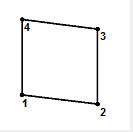
\includegraphics[width=0.3\linewidth]{../Graphics/LISA-quad4.png}
  \caption{quad4 element}
  \label{fig:sub1}
\end{subfigure}%
\begin{subfigure}{.5\textwidth}
  \centering
  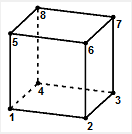
\includegraphics[width=0.3\linewidth]{../Graphics/LISA-hex8.png}
  \caption{hex8 element}
  \label{fig:sub2}
\end{subfigure}
\label{fig:test}
\end{figure}


\begin{figure}[ht]
\centering
\begin{subfigure}{.5\textwidth}
  \centering
  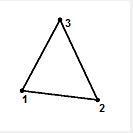
\includegraphics[width=0.3\linewidth]{../Graphics/LISA-tri3.png}
  \caption{Specification for node ordering of tri3 element within LISA}
  \label{fig:sub1}
\end{subfigure}%
\begin{subfigure}{.5\textwidth}
  \centering
  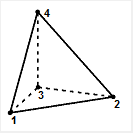
\includegraphics[width=0.3\linewidth]{../Graphics/LISA-tet4.png}
  \caption{tet4 element}
  \label{fig:sub2}
\end{subfigure}
\label{fig:test}
\end{figure}


\begin{figure}[ht]
\centering
\begin{subfigure}{.5\textwidth}
  \centering
  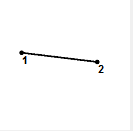
\includegraphics[width=0.3\linewidth]{../Graphics/LISA-line2.png}
  \caption{line2 element}
  \label{fig:sub1}
\end{subfigure}%
\begin{subfigure}{.5\textwidth}
  \centering
  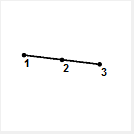
\includegraphics[width=0.3\linewidth]{../Graphics/LISA-line3.png}
  \caption{line3 element}
  \label{fig:sub2}
\end{subfigure}
\label{fig:test}
\end{figure} 

%\section{Calculating Centripetal Force For Paper Mill}
%Assuming a constant speed of the paper mill disk at  the following standard calculation was done to compute a forces that could be specified for different elements in order to simulate the effects on the model.

%F = m $\omega^2$ r\\ 

%where: \\ 
%m - mass of object \\ 
%r - radius from centre \\ 
%$\omega$ - angular velocity (radians per second)

%Using the following values for each variable for the plates forming the outside of the paper mill disk the force could be calculated as:

%mass- paper mill is made of steel with each plate having a volume of approximately $24cm^3$ which gives a mass of
%188 grams


\section{Unit Testing}
%Unit tests to validate the correctness of key functionality



\cite{Centripetal}

\section{Input and output files}
Below can be seen the format of the input files for the system, a LISA .liml and a .json edge definition file\\

\begin{figure}[h!!]
\centering
\begin{subfigure}{.5\textwidth}
  \centering
  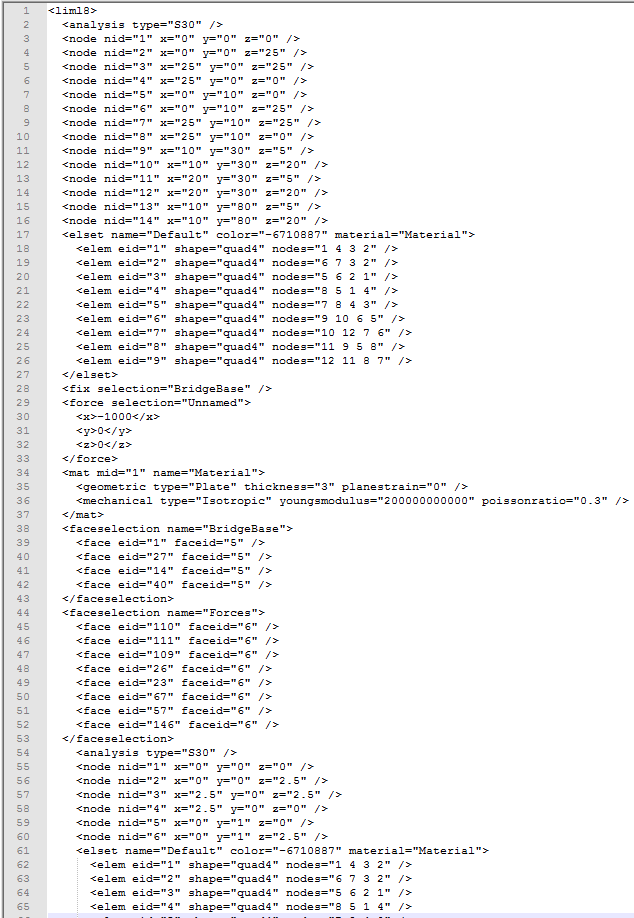
\includegraphics[width=0.6\linewidth]{../Graphics/limlFileLayout.png}
  \caption{Cut down .liml file to show general content which largely defined the schema for the systems data model}
  \label{fig:sub1}
\end{subfigure}%
\begin{subfigure}{.5\textwidth}
  \centering
  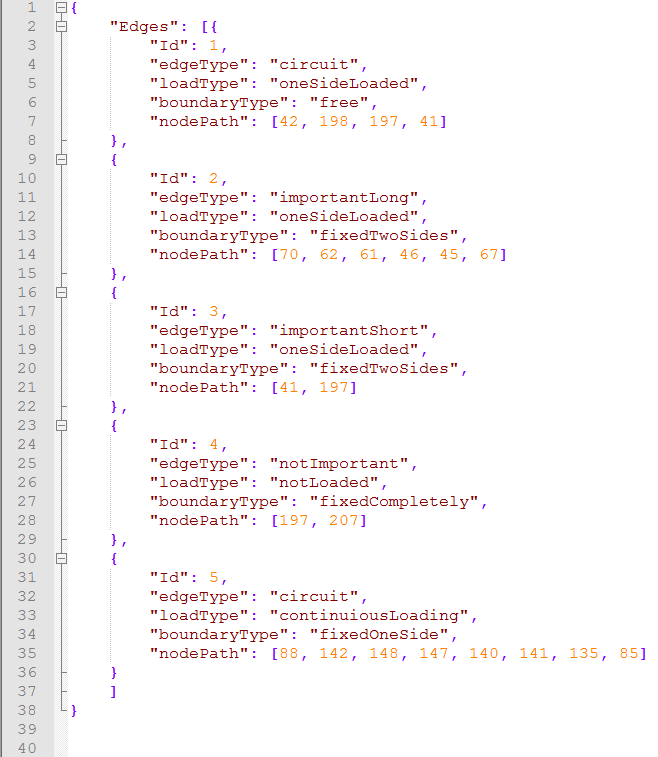
\includegraphics[width=0.8\linewidth]{../Graphics/jsonEdgeFileLayout.png}
  \caption{A json file containing the edges of interest specified by an engineer, this is parsed and the rules are applied to determine the models meshing based on the input}
  \label{fig:sub2}
\end{subfigure}
\label{fig:test}
\end{figure}


\section{Project Layout in Solution Explorer}
Below show the Visual Studio Solution Explorer which provides a general idea of the layout of the project with namespace hierarchies from within an IDE.

\begin{figure}[h!!]
  \centerline{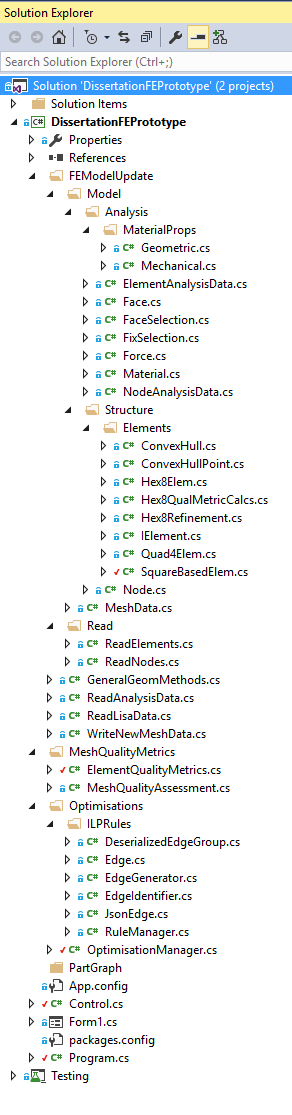
\includegraphics[width=60mm, scale=0.5]{../Graphics/VSolutionExplorer.png}}
  \caption{The metrics calculated by visual studio for all high level modules in the system}
\end{figure}


\section{Software Quality Metrics}
\begin{figure}[h!!]
  \centerline{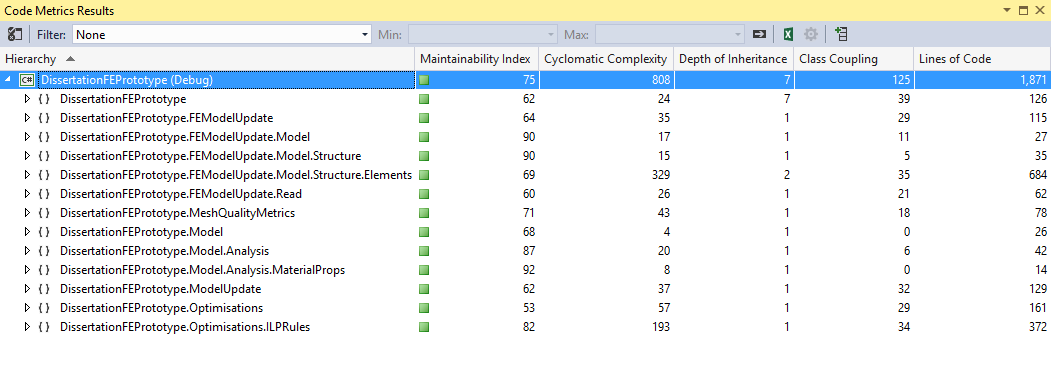
\includegraphics[width=165mm, scale=0.5]{../Graphics/softwareQualityMetrics.png}}
  \caption{The metrics calculated by visual studio for all high level modules in the system}
\end{figure}

\begin{figure}[h!!]
  \centerline{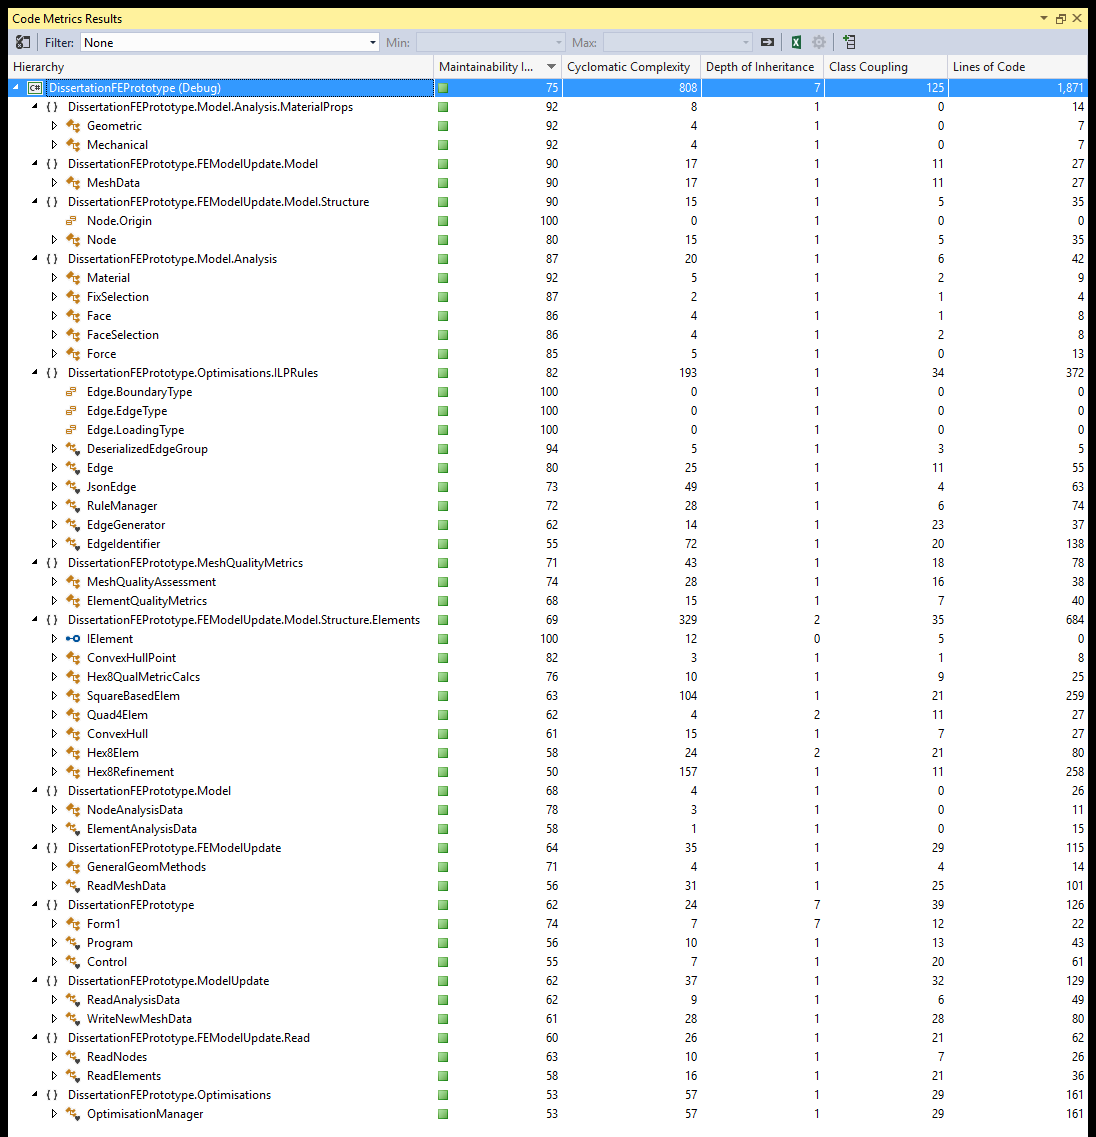
\includegraphics[width=165mm, scale=0.5]{../Graphics/qualityMetricsExpanded.png}}
  \caption{The metrics calculated by visual studio for the all classes in the final system}
\end{figure}
%


\section{Bridge Cross Loading Simulation Results}
Below can be seen the results of executing both the heuristics and the stress refinement method on the suspension bridge model when loads are placed against the base of the bridge in the negative x direction.

\subsection{Heuristic Refinement}

\begin{figure}[h!!]
\centering
\begin{subfigure}{.5\textwidth}
  \centering
	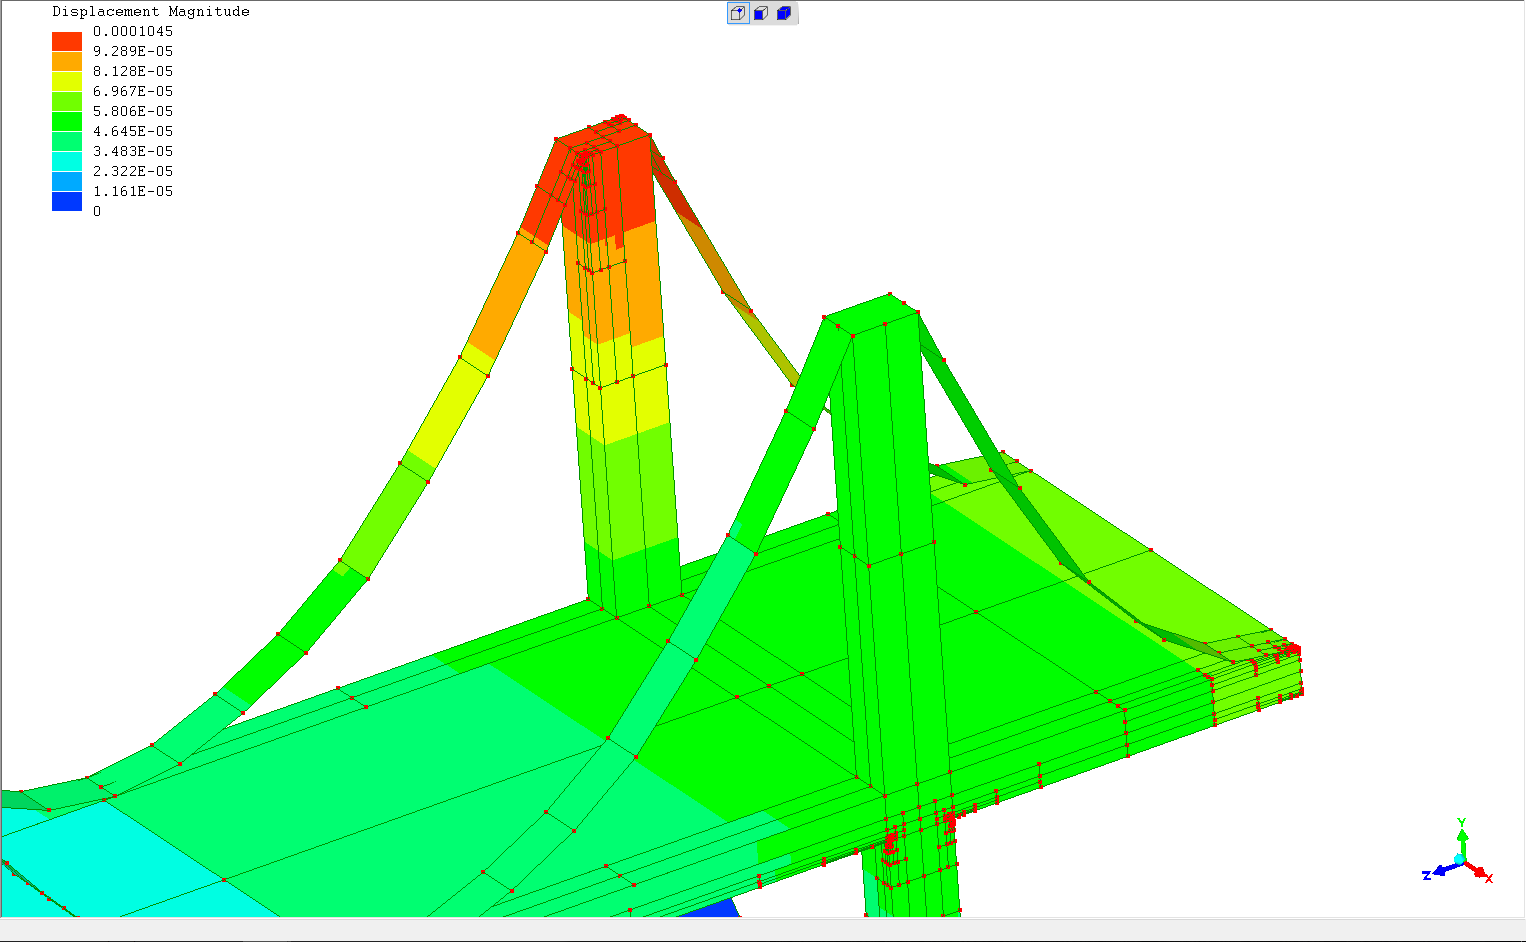
\includegraphics[width=80mm, scale=0.5]{../Graphics/BridgeCrossLoading/bestEdgeSpecResults.png}
  \caption{Important edges specified effectively to facilitate preemptive meshing of area which undergoes high displacement and thus stress}
  \label{fig:sub1}
\end{subfigure}%
\begin{subfigure}{.5\textwidth}
  \centering
  \centerline{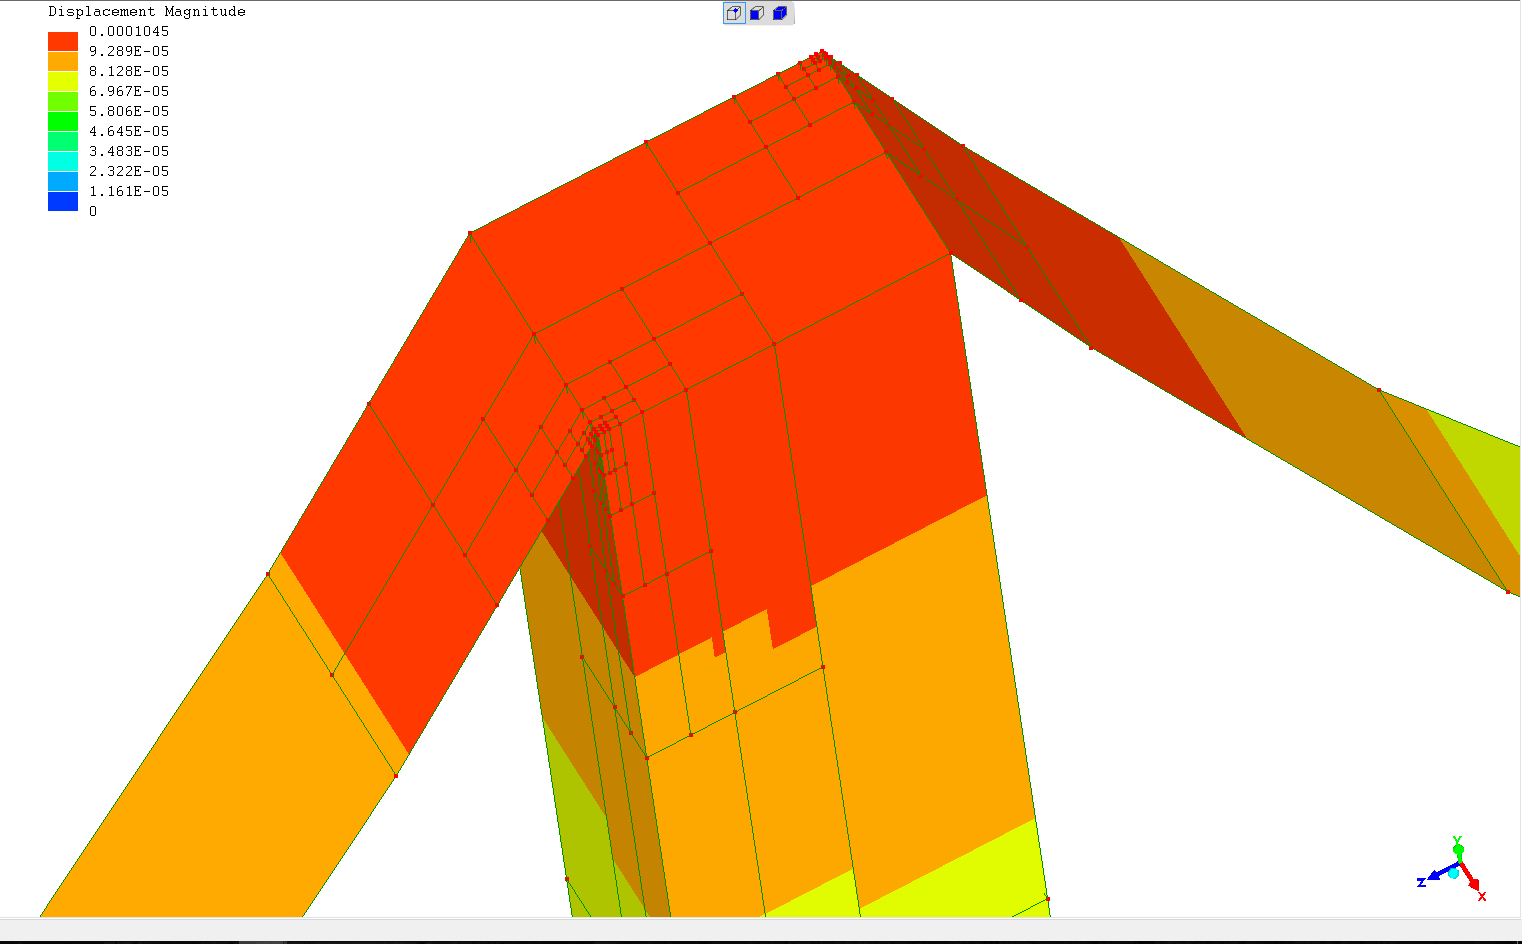
\includegraphics[width=80mm, scale=0.5]{../Graphics/BridgeCrossLoading/bestEdgeSpecResultsCloseUp.png}}
  \caption{Close up view of refinement for high displacement areas }
  \label{fig:sub2}
\end{subfigure}
\label{fig:test}
\end{figure}


\begin{figure}[h!!]
  \centerline{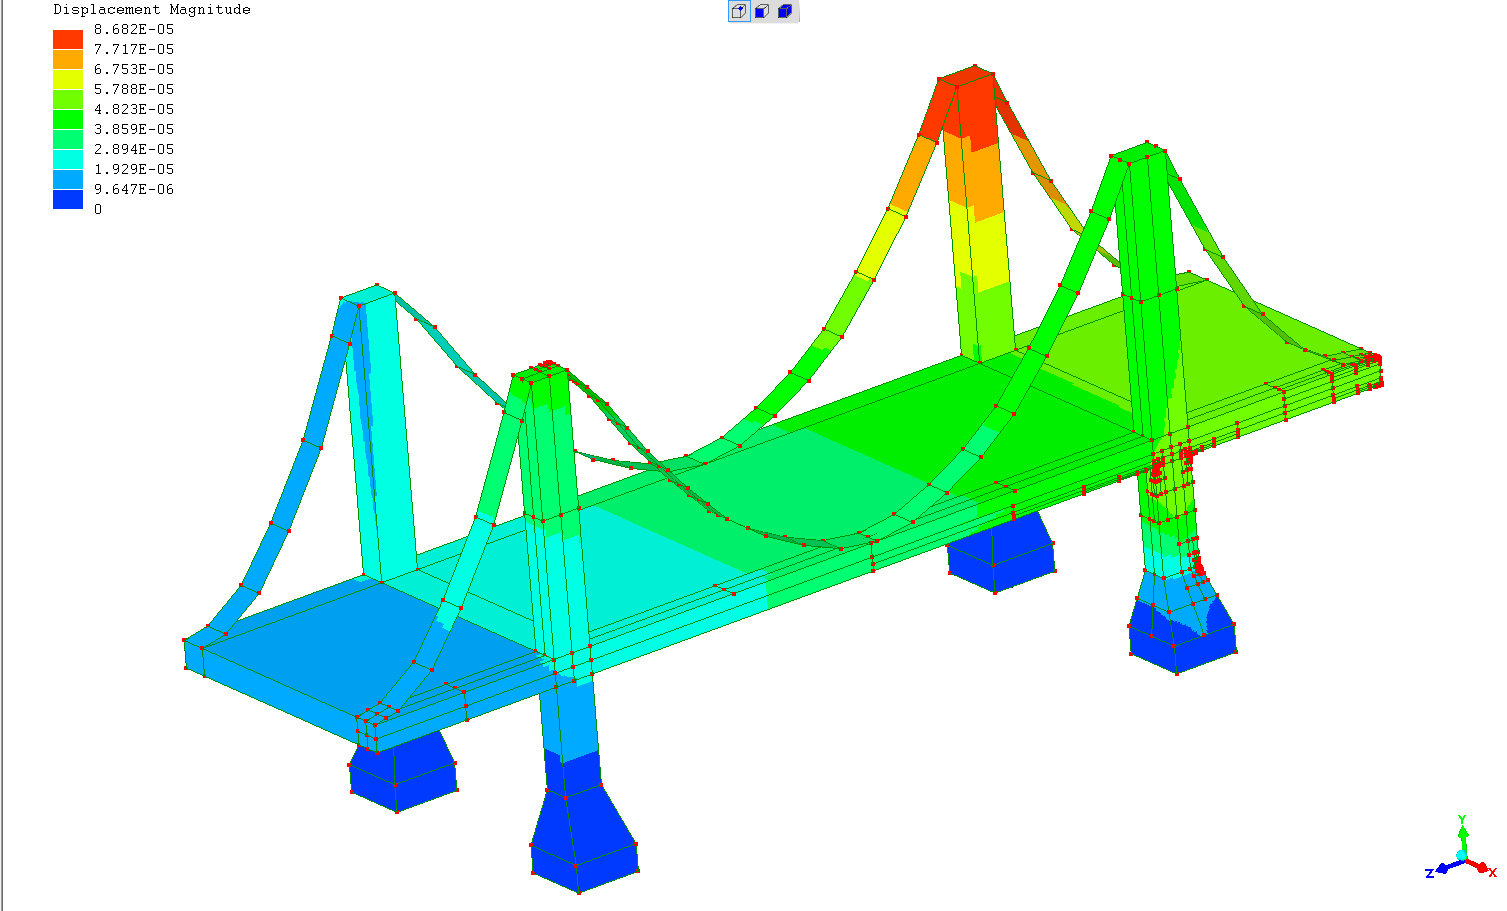
\includegraphics[width=165mm, scale=0.5]{../Graphics/BridgeCrossLoading/okEdgeSpecResults.png}}
  \caption{Important edges more poorly specified missing high displacement region on top of furthest suspension bridge tower}
\end{figure}

\section{Stress Refinement}
\begin{figure}[h!!]
  \centerline{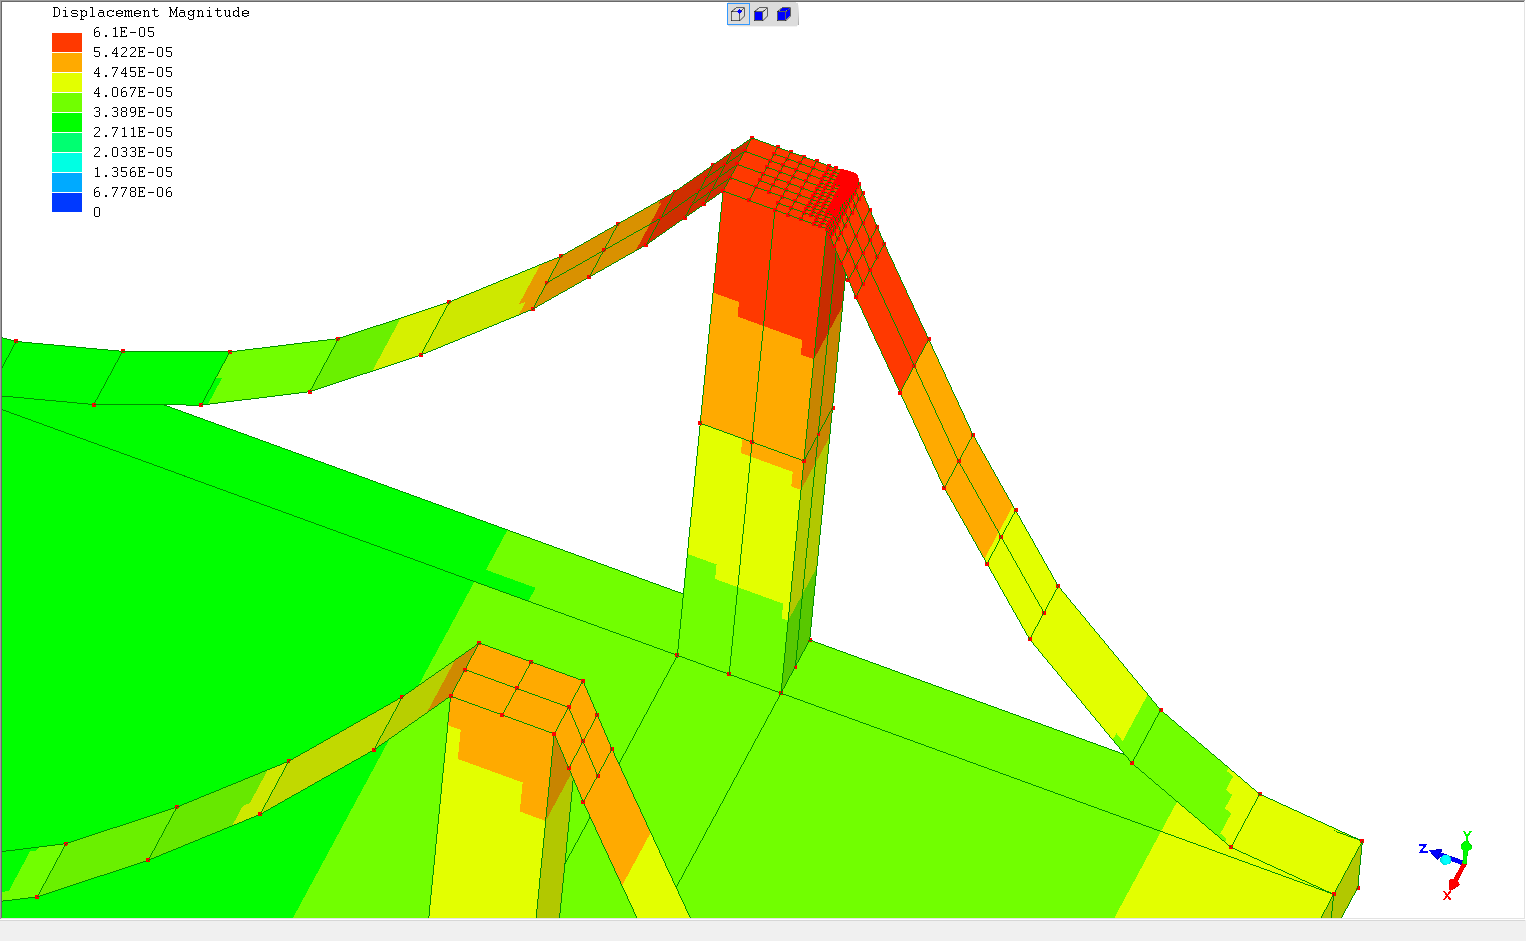
\includegraphics[width=165mm, scale=0.5]{../Graphics/BridgeCrossLoading/the90thPercentileRefinement.png}}
  \caption{Iterative stress/ displacement refinement method used to focus meshing on the top 6\% most displaced region of model}
\end{figure}

\begin{figure}[h!!]
  \centerline{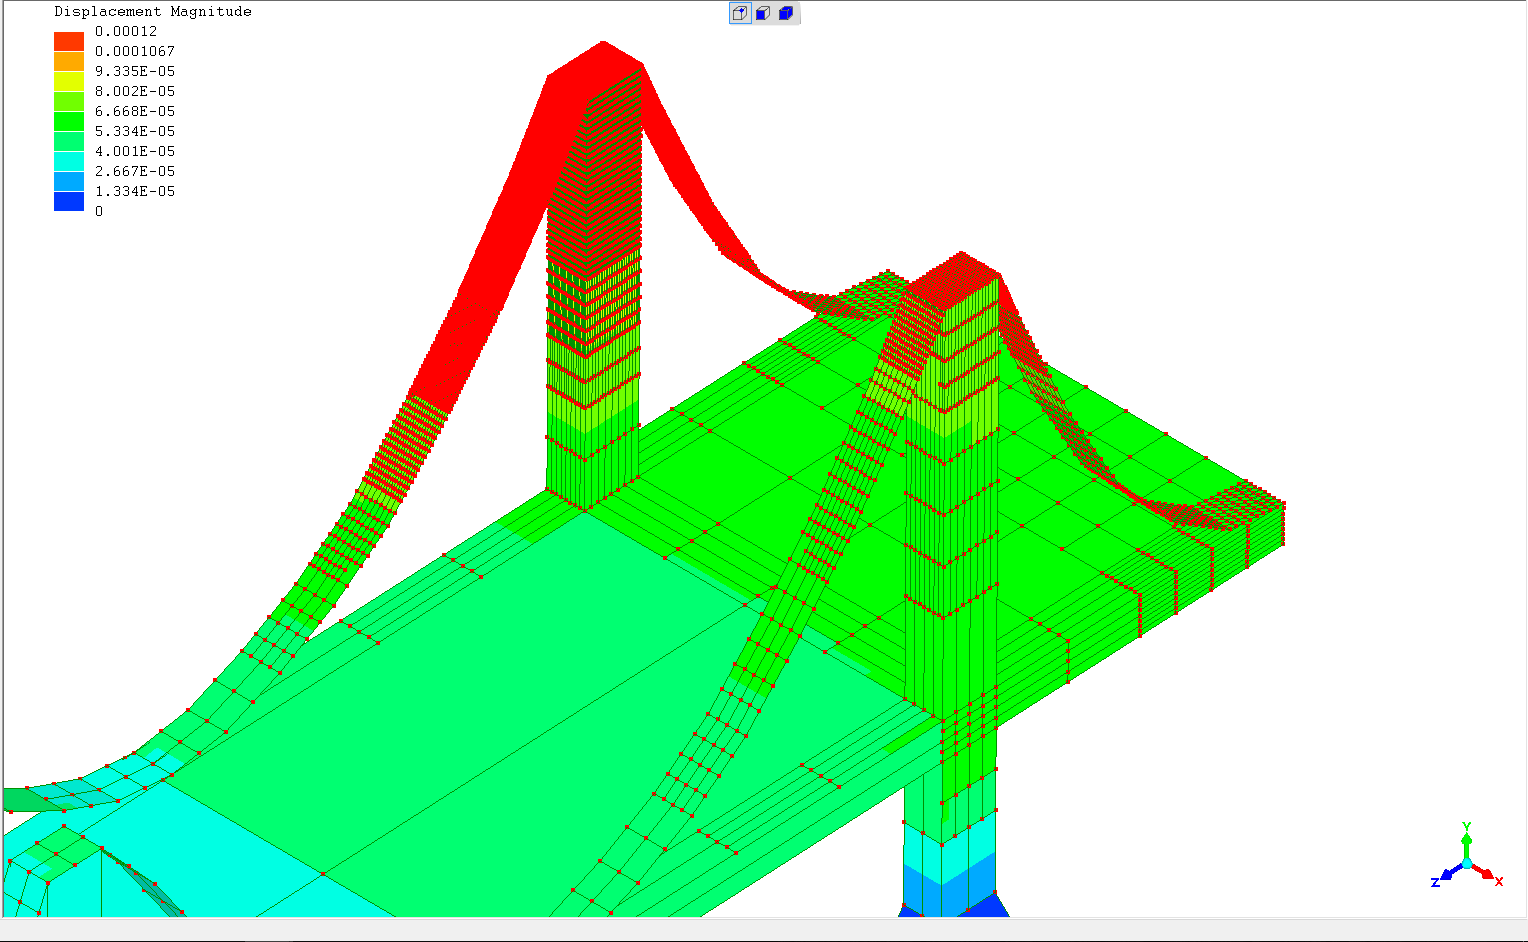
\includegraphics[width=165mm, scale=0.5]{../Graphics/BridgeCrossLoading/aboveAverageRefinement2.png}}
  \caption{Iterative refinement of high displacement but with the remesh threshold specified as the average displacement across the whole model. A consequence of this is the gradient of refinement fidelity that can be seen corresponding to the importance of that part of the structure}
\end{figure}


\begin{figure}[h!!]
  \centerline{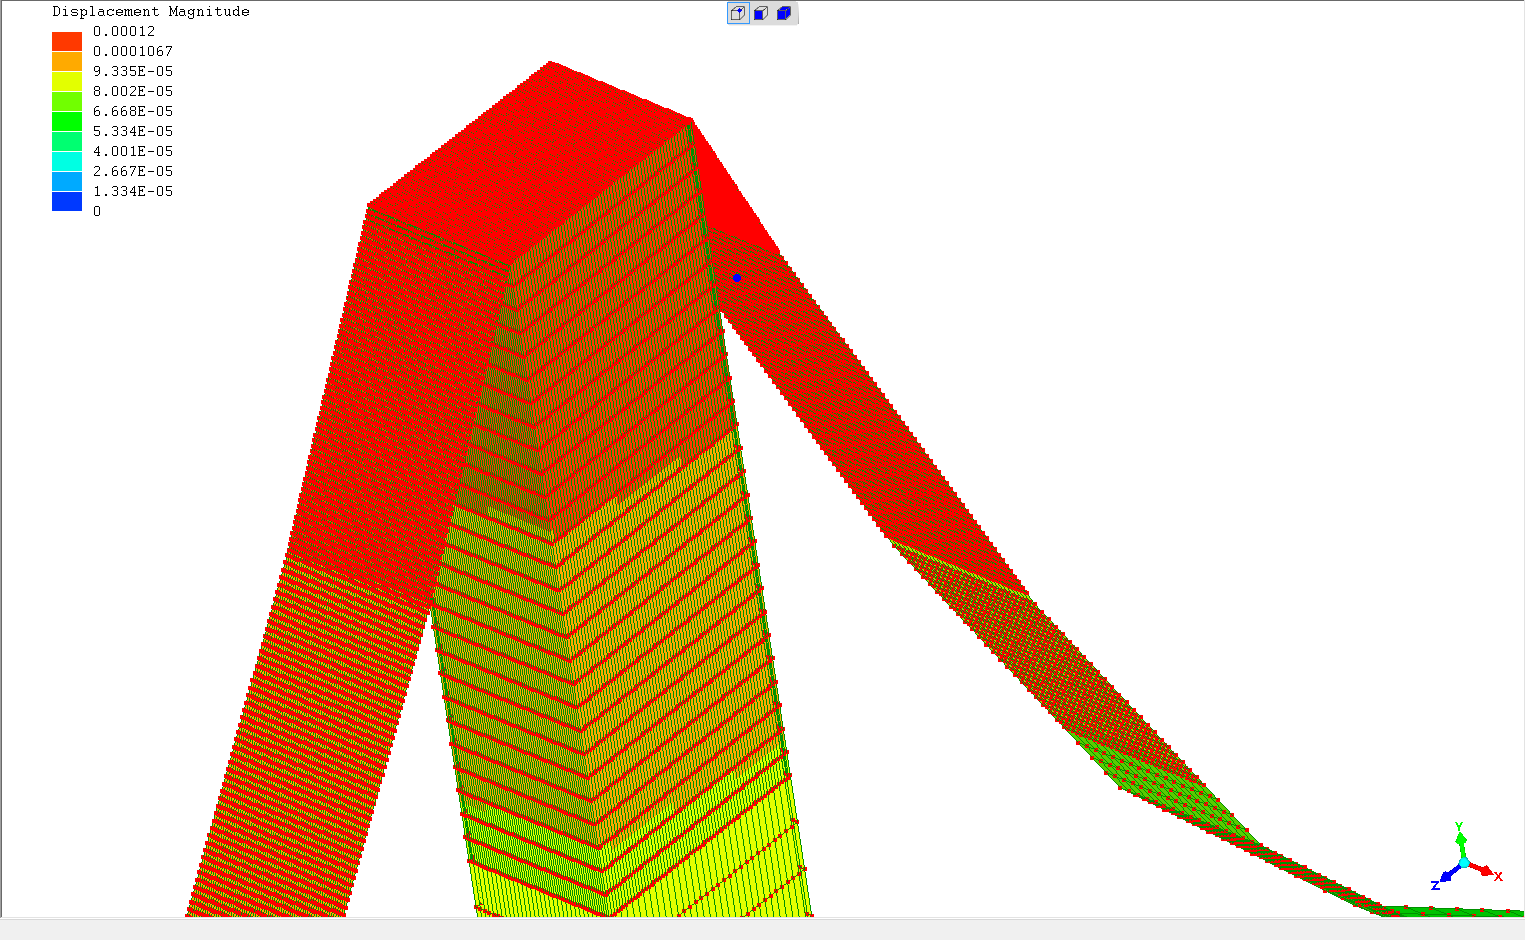
\includegraphics[width=165mm, scale=0.5]{../Graphics/BridgeCrossLoading/aboveAverageRefinement.png}}
  \caption{The metrics calculated by visual studio for the all classes in the final system}
\end{figure}
%\end{changemargin}


\section{Bridge Base Loading Simulation Results}

\section{Paper Mill Simulation Results}

\newpage  
\section{Gantt Chart for Project Time Management}
\pagestyle{empty}
\begin{landscape}
\vspace*{1cm}
\hspace*{-3cm}
\begin{figure}
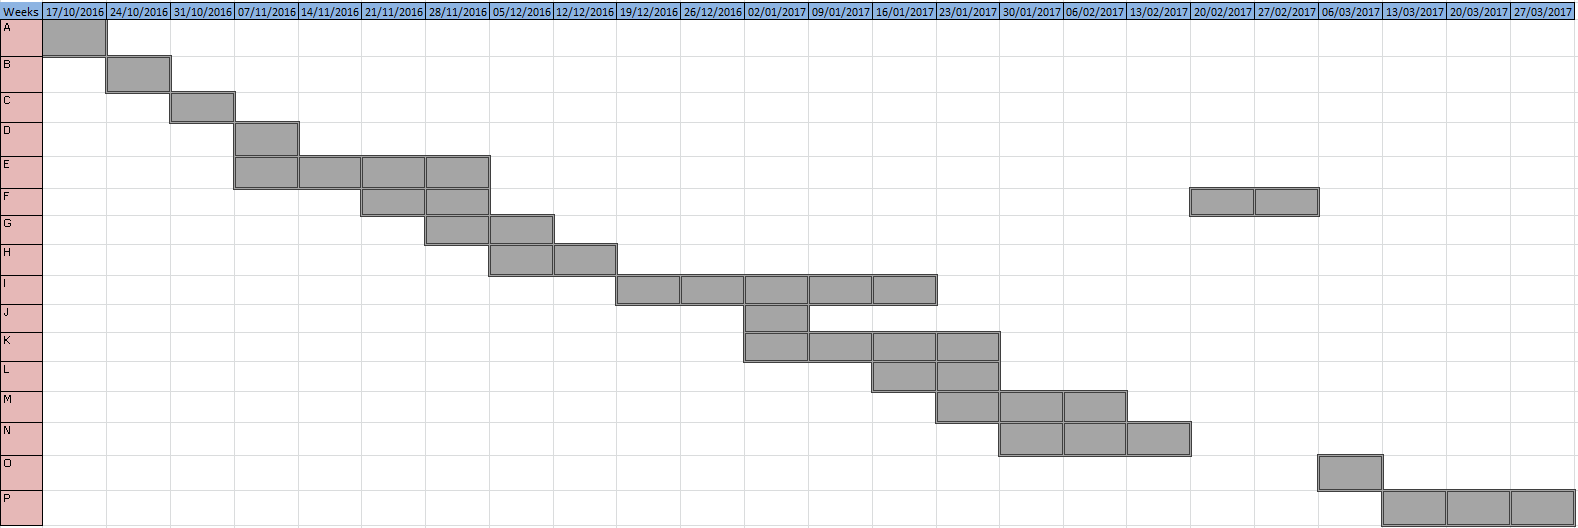
\includegraphics[width =700px, height=300px]{../Graphics/TimePlanUpdated2.png} \par
\end{figure}
\hspace*{-1cm}
\end{landscape}




\end{document}


